% Options for packages loaded elsewhere
\PassOptionsToPackage{unicode}{hyperref}
\PassOptionsToPackage{hyphens}{url}
%
\documentclass[
]{article}
\usepackage{amsmath,amssymb}
\usepackage{iftex}
\ifPDFTeX
  \usepackage[T1]{fontenc}
  \usepackage[utf8]{inputenc}
  \usepackage{textcomp} % provide euro and other symbols
\else % if luatex or xetex
  \usepackage{unicode-math} % this also loads fontspec
  \defaultfontfeatures{Scale=MatchLowercase}
  \defaultfontfeatures[\rmfamily]{Ligatures=TeX,Scale=1}
\fi
\usepackage{lmodern}
\ifPDFTeX\else
  % xetex/luatex font selection
\fi
% Use upquote if available, for straight quotes in verbatim environments
\IfFileExists{upquote.sty}{\usepackage{upquote}}{}
\IfFileExists{microtype.sty}{% use microtype if available
  \usepackage[]{microtype}
  \UseMicrotypeSet[protrusion]{basicmath} % disable protrusion for tt fonts
}{}
\makeatletter
\@ifundefined{KOMAClassName}{% if non-KOMA class
  \IfFileExists{parskip.sty}{%
    \usepackage{parskip}
  }{% else
    \setlength{\parindent}{0pt}
    \setlength{\parskip}{6pt plus 2pt minus 1pt}}
}{% if KOMA class
  \KOMAoptions{parskip=half}}
\makeatother
\usepackage{xcolor}
\usepackage[margin=1in]{geometry}
\usepackage{color}
\usepackage{fancyvrb}
\newcommand{\VerbBar}{|}
\newcommand{\VERB}{\Verb[commandchars=\\\{\}]}
\DefineVerbatimEnvironment{Highlighting}{Verbatim}{commandchars=\\\{\}}
% Add ',fontsize=\small' for more characters per line
\usepackage{framed}
\definecolor{shadecolor}{RGB}{248,248,248}
\newenvironment{Shaded}{\begin{snugshade}}{\end{snugshade}}
\newcommand{\AlertTok}[1]{\textcolor[rgb]{0.94,0.16,0.16}{#1}}
\newcommand{\AnnotationTok}[1]{\textcolor[rgb]{0.56,0.35,0.01}{\textbf{\textit{#1}}}}
\newcommand{\AttributeTok}[1]{\textcolor[rgb]{0.13,0.29,0.53}{#1}}
\newcommand{\BaseNTok}[1]{\textcolor[rgb]{0.00,0.00,0.81}{#1}}
\newcommand{\BuiltInTok}[1]{#1}
\newcommand{\CharTok}[1]{\textcolor[rgb]{0.31,0.60,0.02}{#1}}
\newcommand{\CommentTok}[1]{\textcolor[rgb]{0.56,0.35,0.01}{\textit{#1}}}
\newcommand{\CommentVarTok}[1]{\textcolor[rgb]{0.56,0.35,0.01}{\textbf{\textit{#1}}}}
\newcommand{\ConstantTok}[1]{\textcolor[rgb]{0.56,0.35,0.01}{#1}}
\newcommand{\ControlFlowTok}[1]{\textcolor[rgb]{0.13,0.29,0.53}{\textbf{#1}}}
\newcommand{\DataTypeTok}[1]{\textcolor[rgb]{0.13,0.29,0.53}{#1}}
\newcommand{\DecValTok}[1]{\textcolor[rgb]{0.00,0.00,0.81}{#1}}
\newcommand{\DocumentationTok}[1]{\textcolor[rgb]{0.56,0.35,0.01}{\textbf{\textit{#1}}}}
\newcommand{\ErrorTok}[1]{\textcolor[rgb]{0.64,0.00,0.00}{\textbf{#1}}}
\newcommand{\ExtensionTok}[1]{#1}
\newcommand{\FloatTok}[1]{\textcolor[rgb]{0.00,0.00,0.81}{#1}}
\newcommand{\FunctionTok}[1]{\textcolor[rgb]{0.13,0.29,0.53}{\textbf{#1}}}
\newcommand{\ImportTok}[1]{#1}
\newcommand{\InformationTok}[1]{\textcolor[rgb]{0.56,0.35,0.01}{\textbf{\textit{#1}}}}
\newcommand{\KeywordTok}[1]{\textcolor[rgb]{0.13,0.29,0.53}{\textbf{#1}}}
\newcommand{\NormalTok}[1]{#1}
\newcommand{\OperatorTok}[1]{\textcolor[rgb]{0.81,0.36,0.00}{\textbf{#1}}}
\newcommand{\OtherTok}[1]{\textcolor[rgb]{0.56,0.35,0.01}{#1}}
\newcommand{\PreprocessorTok}[1]{\textcolor[rgb]{0.56,0.35,0.01}{\textit{#1}}}
\newcommand{\RegionMarkerTok}[1]{#1}
\newcommand{\SpecialCharTok}[1]{\textcolor[rgb]{0.81,0.36,0.00}{\textbf{#1}}}
\newcommand{\SpecialStringTok}[1]{\textcolor[rgb]{0.31,0.60,0.02}{#1}}
\newcommand{\StringTok}[1]{\textcolor[rgb]{0.31,0.60,0.02}{#1}}
\newcommand{\VariableTok}[1]{\textcolor[rgb]{0.00,0.00,0.00}{#1}}
\newcommand{\VerbatimStringTok}[1]{\textcolor[rgb]{0.31,0.60,0.02}{#1}}
\newcommand{\WarningTok}[1]{\textcolor[rgb]{0.56,0.35,0.01}{\textbf{\textit{#1}}}}
\usepackage{graphicx}
\makeatletter
\def\maxwidth{\ifdim\Gin@nat@width>\linewidth\linewidth\else\Gin@nat@width\fi}
\def\maxheight{\ifdim\Gin@nat@height>\textheight\textheight\else\Gin@nat@height\fi}
\makeatother
% Scale images if necessary, so that they will not overflow the page
% margins by default, and it is still possible to overwrite the defaults
% using explicit options in \includegraphics[width, height, ...]{}
\setkeys{Gin}{width=\maxwidth,height=\maxheight,keepaspectratio}
% Set default figure placement to htbp
\makeatletter
\def\fps@figure{htbp}
\makeatother
\setlength{\emergencystretch}{3em} % prevent overfull lines
\providecommand{\tightlist}{%
  \setlength{\itemsep}{0pt}\setlength{\parskip}{0pt}}
\setcounter{secnumdepth}{-\maxdimen} % remove section numbering
\ifLuaTeX
  \usepackage{selnolig}  % disable illegal ligatures
\fi
\IfFileExists{bookmark.sty}{\usepackage{bookmark}}{\usepackage{hyperref}}
\IfFileExists{xurl.sty}{\usepackage{xurl}}{} % add URL line breaks if available
\urlstyle{same}
\hypersetup{
  pdftitle={Projet sur le Logiciel R \& Studio},
  pdfauthor={COMPAORE Mohamadi Bassirou \& Samson Awouto \& Diop Yague},
  hidelinks,
  pdfcreator={LaTeX via pandoc}}

\title{Projet sur le Logiciel R \& Studio}
\author{COMPAORE Mohamadi Bassirou \& Samson Awouto \& Diop Yague}
\date{2024-06-01}

\begin{document}
\maketitle

{
\setcounter{tocdepth}{3}
\tableofcontents
}
\hypertarget{ruxe9solution-des-uxe9quations-non-linuxe9aires-avec-le-logiciel-r}{%
\section{Résolution des équations non linéaires avec le logiciel
R}\label{ruxe9solution-des-uxe9quations-non-linuxe9aires-avec-le-logiciel-r}}

\hypertarget{rstudio-est-un-environnement-de-duxe9veloppement-gratuit-libre-et-multiplateforme-pour-r-un-langage-de-programmation-utilisuxe9-pour-le-traitement-de-donnuxe9es-et-lanalyse-statistique.dans-notre-contextenous-allons-utiliser-rstudio-poour-la-ruxe9solution-des-uxe9quations-non-linuxe9aire.les-uxe9quations-non-linuxe9aires-sont-des-uxe9quations-dont-le-degruxe9-est-supuxe9rieure-uxe0-1}{%
\subsubsection{RStudio est un environnement de développement gratuit,
libre et multiplateforme pour R, un langage de programmation utilisé
pour le traitement de données et l'analyse statistique.Dans notre
contexte,nous allons utiliser RStudio poour la résolution des équations
non linéaire.Les équations non linéaires sont des équations dont le
degré est supérieure à
1}\label{rstudio-est-un-environnement-de-duxe9veloppement-gratuit-libre-et-multiplateforme-pour-r-un-langage-de-programmation-utilisuxe9-pour-le-traitement-de-donnuxe9es-et-lanalyse-statistique.dans-notre-contextenous-allons-utiliser-rstudio-poour-la-ruxe9solution-des-uxe9quations-non-linuxe9aire.les-uxe9quations-non-linuxe9aires-sont-des-uxe9quations-dont-le-degruxe9-est-supuxe9rieure-uxe0-1}}

\hypertarget{installation-et-importation-des-packages}{%
\subsection{Installation et Importation des
Packages}\label{installation-et-importation-des-packages}}

\begin{Shaded}
\begin{Highlighting}[]
\CommentTok{\# Installer et charger le  lpSolve}
\CommentTok{\#install.packages}
\CommentTok{\#install.packages("rootSolve")}
\CommentTok{\#install.packages("nleqslv")}
\FunctionTok{library}\NormalTok{(lpSolve)}
\FunctionTok{library}\NormalTok{(haven)}
\FunctionTok{library}\NormalTok{(nleqslv)}
\FunctionTok{library}\NormalTok{(rootSolve)}
\FunctionTok{library}\NormalTok{(magrittr)}
\FunctionTok{library}\NormalTok{(dplyr)}
\end{Highlighting}
\end{Shaded}

\begin{verbatim}
## 
## Attachement du package : 'dplyr'
\end{verbatim}

\begin{verbatim}
## Les objets suivants sont masqués depuis 'package:stats':
## 
##     filter, lag
\end{verbatim}

\begin{verbatim}
## Les objets suivants sont masqués depuis 'package:base':
## 
##     intersect, setdiff, setequal, union
\end{verbatim}

\begin{Shaded}
\begin{Highlighting}[]
\FunctionTok{library}\NormalTok{(tidyr)}
\end{Highlighting}
\end{Shaded}

\begin{verbatim}
## 
## Attachement du package : 'tidyr'
\end{verbatim}

\begin{verbatim}
## L'objet suivant est masqué depuis 'package:magrittr':
## 
##     extract
\end{verbatim}

\begin{Shaded}
\begin{Highlighting}[]
\FunctionTok{library}\NormalTok{(rootSolve)}
\FunctionTok{library}\NormalTok{(nleqslv)}
\FunctionTok{library}\NormalTok{(pracma)}
\end{Highlighting}
\end{Shaded}

\begin{verbatim}
## 
## Attachement du package : 'pracma'
\end{verbatim}

\begin{verbatim}
## Les objets suivants sont masqués depuis 'package:magrittr':
## 
##     and, mod, or
\end{verbatim}

\begin{verbatim}
## Les objets suivants sont masqués depuis 'package:rootSolve':
## 
##     gradient, hessian
\end{verbatim}

\begin{Shaded}
\begin{Highlighting}[]
\FunctionTok{library}\NormalTok{(stats)}
\FunctionTok{library}\NormalTok{(reshape)}
\end{Highlighting}
\end{Shaded}

\begin{verbatim}
## 
## Attachement du package : 'reshape'
\end{verbatim}

\begin{verbatim}
## Les objets suivants sont masqués depuis 'package:tidyr':
## 
##     expand, smiths
\end{verbatim}

\begin{verbatim}
## L'objet suivant est masqué depuis 'package:dplyr':
## 
##     rename
\end{verbatim}

\begin{Shaded}
\begin{Highlighting}[]
\FunctionTok{library}\NormalTok{(ggplot2)}
\FunctionTok{library}\NormalTok{(deSolve)}
\end{Highlighting}
\end{Shaded}

\begin{verbatim}
## 
## Attachement du package : 'deSolve'
\end{verbatim}

\begin{verbatim}
## L'objet suivant est masqué depuis 'package:pracma':
## 
##     rk4
\end{verbatim}

\hypertarget{pruxe9sentation-des-differents-packages}{%
\section{Présentation des differents
packages}\label{pruxe9sentation-des-differents-packages}}

\hypertarget{dans-cette-partie-nous-mettons-en-en-exergue-les-packages-nuxe9cessaires-uxe0-la-resolution-des-uxe9quations-non-linuxe9aires.lobjectif-finale-est-de-pouvoir-optimiser-nos-differentes-donnuxe9es-en-fonction-du-besoin.-nous-pouvons-par-exemples-optimiser-les-couts-de-production-dune-entrepriseles-duxe9penses-publiques-de-letatles-profits-dune-entreprise-etc}{%
\subsubsection{Dans cette partie, nous mettons en en exergue les
packages nécessaires à la resolution des équations non
linéaires.L'Objectif finale est de pouvoir optimiser nos differentes
données en fonction du besoin. Nous pouvons par exemples optimiser les
couts de production d'une entreprise,les dépenses publiques de
l'Etat,les profits d'une entreprise
etc\ldots{}}\label{dans-cette-partie-nous-mettons-en-en-exergue-les-packages-nuxe9cessaires-uxe0-la-resolution-des-uxe9quations-non-linuxe9aires.lobjectif-finale-est-de-pouvoir-optimiser-nos-differentes-donnuxe9es-en-fonction-du-besoin.-nous-pouvons-par-exemples-optimiser-les-couts-de-production-dune-entrepriseles-duxe9penses-publiques-de-letatles-profits-dune-entreprise-etc}}

\hypertarget{utilisation-du-package-rootsolve}{%
\subsection{Utilisation du Package
``rootSolve''}\label{utilisation-du-package-rootsolve}}

\begin{Shaded}
\begin{Highlighting}[]
\CommentTok{\# Chargement du package}

\CommentTok{\# Définition du système d\textquotesingle{}équations}
\NormalTok{equations }\OtherTok{\textless{}{-}} \ControlFlowTok{function}\NormalTok{(x) \{}
  \CommentTok{\# Définition des équations du système}
\NormalTok{  equation\_1 }\OtherTok{\textless{}{-}} \DecValTok{3}\SpecialCharTok{*}\NormalTok{x[}\DecValTok{1}\NormalTok{]}\SpecialCharTok{\^{}}\DecValTok{2} \SpecialCharTok{+}\NormalTok{ x[}\DecValTok{2}\NormalTok{]}\SpecialCharTok{\^{}}\DecValTok{2} \SpecialCharTok{{-}} \DecValTok{1}    
\NormalTok{  equation\_2 }\OtherTok{\textless{}{-}} \DecValTok{5}\SpecialCharTok{*}\NormalTok{x[}\DecValTok{1}\NormalTok{]}\SpecialCharTok{\^{}}\DecValTok{2} \SpecialCharTok{{-}} \DecValTok{2}\SpecialCharTok{*}\NormalTok{x[}\DecValTok{2}\NormalTok{]}\SpecialCharTok{\^{}}\DecValTok{2} \SpecialCharTok{+} \DecValTok{4}
                              
  \CommentTok{\# Retourner les équations sous forme de vecteur}
  \FunctionTok{return}\NormalTok{(}\FunctionTok{c}\NormalTok{(equation\_1, equation\_2))}
\NormalTok{\}}

\CommentTok{\# Vecteur initial de valeurs approchées pour les variables}
\NormalTok{point\_de\_départ }\OtherTok{\textless{}{-}} \FunctionTok{c}\NormalTok{(}\DecValTok{1}\NormalTok{, }\DecValTok{1}\NormalTok{)}

\CommentTok{\# Résolution du système d\textquotesingle{}équations non linéaires}
\NormalTok{solution }\OtherTok{\textless{}{-}} \FunctionTok{multiroot}\NormalTok{(}\AttributeTok{f =}\NormalTok{ equations, }\AttributeTok{start =}\NormalTok{ point\_de\_départ)}

\CommentTok{\# Affichage des solutions}
\FunctionTok{print}\NormalTok{(solution}\SpecialCharTok{$}\NormalTok{root)}
\end{Highlighting}
\end{Shaded}

\begin{verbatim}
## [1] 0.05274924 1.24316312
\end{verbatim}

\begin{Shaded}
\begin{Highlighting}[]
\CommentTok{\# AUTRES ARGUMENTS}
           \CommentTok{\#tolerance =  : pour définir une tolérance plus stricte pour la convergence.}
            \CommentTok{\#maxiter: pour spécifier le nombre maximal d\textquotesingle{}itérations autorisées}
\end{Highlighting}
\end{Shaded}

\hypertarget{utilisation-du-package-nleqslv}{%
\subsection{Utilisation du Package
``nleqslv''}\label{utilisation-du-package-nleqslv}}

\begin{Shaded}
\begin{Highlighting}[]
\CommentTok{\# Chargement du package nleqslv}

\CommentTok{\# Définition de la fonction du système d\textquotesingle{}équations}
\NormalTok{systeme\_equations }\OtherTok{\textless{}{-}} \ControlFlowTok{function}\NormalTok{(x) \{}
\NormalTok{  eq1 }\OtherTok{\textless{}{-}} \DecValTok{3}\SpecialCharTok{*}\NormalTok{x[}\DecValTok{1}\NormalTok{]}\SpecialCharTok{\^{}}\DecValTok{2} \SpecialCharTok{+}\NormalTok{ x[}\DecValTok{2}\NormalTok{]}\SpecialCharTok{\^{}}\DecValTok{2} \SpecialCharTok{{-}} \DecValTok{1}
\NormalTok{  eq2 }\OtherTok{\textless{}{-}} \DecValTok{5}\SpecialCharTok{*}\NormalTok{x[}\DecValTok{1}\NormalTok{]}\SpecialCharTok{\^{}}\DecValTok{2} \SpecialCharTok{{-}} \DecValTok{2}\SpecialCharTok{*}\NormalTok{x[}\DecValTok{2}\NormalTok{]}\SpecialCharTok{\^{}}\DecValTok{2} \SpecialCharTok{+} \DecValTok{4}
  \FunctionTok{return}\NormalTok{(}\FunctionTok{c}\NormalTok{(eq1, eq2))}
\NormalTok{\}}

\CommentTok{\# Résolution du système d\textquotesingle{}équations avec la méthode de Newton}
\NormalTok{solution }\OtherTok{\textless{}{-}} \FunctionTok{nleqslv}\NormalTok{(}\FunctionTok{c}\NormalTok{(}\DecValTok{1}\NormalTok{, }\DecValTok{1}\NormalTok{), }
\NormalTok{                    systeme\_equations, }
                    \AttributeTok{method =} \StringTok{"Newton"}\NormalTok{)}

\CommentTok{\# Affichage des solutions}
\FunctionTok{print}\NormalTok{(solution}\SpecialCharTok{$}\NormalTok{x)}
\end{Highlighting}
\end{Shaded}

\begin{verbatim}
## [1] 0.0001561915 1.3416407895
\end{verbatim}

\begin{Shaded}
\begin{Highlighting}[]
\CommentTok{\# afficher l\textquotesingle{}intervalle de validité de la solution}

\FunctionTok{print}\NormalTok{(solution}\SpecialCharTok{$}\NormalTok{fvec) }
\end{Highlighting}
\end{Shaded}

\begin{verbatim}
## [1] 0.8000001 0.4000001
\end{verbatim}

\begin{Shaded}
\begin{Highlighting}[]
\DocumentationTok{\#\# afficher le nombre d\textquotesingle{}ittération}
\FunctionTok{print}\NormalTok{(solution}\SpecialCharTok{$}\NormalTok{iter)}
\end{Highlighting}
\end{Shaded}

\begin{verbatim}
## [1] 11
\end{verbatim}

\hypertarget{utilisation-du-package-pracma}{%
\subsection{Utilisation du Package
``pracma''}\label{utilisation-du-package-pracma}}

\begin{Shaded}
\begin{Highlighting}[]
\CommentTok{\# Définition du système d\textquotesingle{}équations}
\NormalTok{equations }\OtherTok{\textless{}{-}} \ControlFlowTok{function}\NormalTok{(x) \{}
\NormalTok{  pracma\_1 }\OtherTok{\textless{}{-}}\NormalTok{ x[}\DecValTok{1}\NormalTok{]}\SpecialCharTok{\^{}}\DecValTok{2} \SpecialCharTok{+}\NormalTok{ x[}\DecValTok{2}\NormalTok{]}\SpecialCharTok{\^{}}\DecValTok{2} \SpecialCharTok{+}\DecValTok{200}
\NormalTok{  pracma\_2 }\OtherTok{\textless{}{-}}\NormalTok{ x[}\DecValTok{1}\NormalTok{]}\SpecialCharTok{\^{}}\DecValTok{2} \SpecialCharTok{{-}}\NormalTok{ x[}\DecValTok{2}\NormalTok{]}\SpecialCharTok{\^{}}\DecValTok{2} \SpecialCharTok{{-}}\DecValTok{1000}
  \FunctionTok{return}\NormalTok{(}\FunctionTok{c}\NormalTok{(pracma\_1, pracma\_2))}
\NormalTok{\}}

\CommentTok{\# Spécification des valeurs initiales pour les variables}
\NormalTok{initial\_guess }\OtherTok{\textless{}{-}} \FunctionTok{c}\NormalTok{(}\DecValTok{1}\NormalTok{, }\DecValTok{1}\NormalTok{)}

\CommentTok{\# Résolution du système d\textquotesingle{}équations non linéaires}
\NormalTok{solution }\OtherTok{\textless{}{-}} \FunctionTok{fsolve}\NormalTok{(equations, initial\_guess)}

\CommentTok{\# Affichage des solutions}
\FunctionTok{print}\NormalTok{(solution)}
\end{Highlighting}
\end{Shaded}

\begin{verbatim}
## $x
## [1] -20.000000   1.043737
## 
## $fval
## [1]  601.0894 -601.0894
\end{verbatim}

\hypertarget{utilisation-du-package-stats}{%
\subsection{Utilisation du Package
``stats''}\label{utilisation-du-package-stats}}

\begin{Shaded}
\begin{Highlighting}[]
\CommentTok{\# Définition de la fonction d\textquotesingle{}utilité et de la contrainte budgétaire}
\NormalTok{utilite }\OtherTok{\textless{}{-}} \ControlFlowTok{function}\NormalTok{(x) \{}
\NormalTok{  utilité }\OtherTok{\textless{}{-}} \SpecialCharTok{{-}}\NormalTok{ (x[}\DecValTok{1}\NormalTok{]}\SpecialCharTok{\^{}}\DecValTok{2} \SpecialCharTok{+}\NormalTok{ x[}\DecValTok{2}\NormalTok{]}\SpecialCharTok{\^{}}\DecValTok{2}\NormalTok{)}
  \FunctionTok{return}\NormalTok{(utilité)}
\NormalTok{\}}

\NormalTok{contrainte\_budg }\OtherTok{\textless{}{-}} \ControlFlowTok{function}\NormalTok{(x) \{}
\NormalTok{  revenu\_total }\OtherTok{\textless{}{-}} \SpecialCharTok{{-}}\DecValTok{1000} \SpecialCharTok{+}\NormalTok{x[}\DecValTok{1}\NormalTok{] }\SpecialCharTok{+}\NormalTok{ x[}\DecValTok{2}\NormalTok{] }
  \FunctionTok{return}\NormalTok{(revenu\_total)}
\NormalTok{\}}

\CommentTok{\# Fonction objectif (utilité sous contrainte)}
\NormalTok{fonction\_objectif }\OtherTok{\textless{}{-}} \ControlFlowTok{function}\NormalTok{(x\_lambda) \{}
\NormalTok{  x }\OtherTok{\textless{}{-}}\NormalTok{ x\_lambda[}\DecValTok{1}\SpecialCharTok{:}\DecValTok{2}\NormalTok{]}
\NormalTok{  lambda }\OtherTok{\textless{}{-}}\NormalTok{ x\_lambda[}\DecValTok{3}\NormalTok{]}
  \FunctionTok{return}\NormalTok{((}\FunctionTok{utilite}\NormalTok{(x) }\SpecialCharTok{{-}}\NormalTok{ lambda }\SpecialCharTok{*} \FunctionTok{contrainte\_budg}\NormalTok{(x)))}
\NormalTok{\}}

\CommentTok{\# Variables initiales}
\NormalTok{x0 }\OtherTok{\textless{}{-}} \FunctionTok{c}\NormalTok{(}\DecValTok{0}\NormalTok{, }\DecValTok{0}\NormalTok{)  }\CommentTok{\# Valeurs initiales pour x1 et x2}
\NormalTok{lambda0 }\OtherTok{\textless{}{-}} \DecValTok{1}        \CommentTok{\# Valeur initiale de lambda}

\CommentTok{\# Résolution du problème d\textquotesingle{}optimisation}
\NormalTok{resultat }\OtherTok{\textless{}{-}} \FunctionTok{optim}\NormalTok{(}\FunctionTok{c}\NormalTok{(x0, lambda0), fonction\_objectif, }\AttributeTok{method =} \StringTok{"BFGS"}\NormalTok{)}

\CommentTok{\# Affichage des résultats}
\NormalTok{x\_opt }\OtherTok{\textless{}{-}}\NormalTok{ resultat}\SpecialCharTok{$}\NormalTok{par[}\DecValTok{1}\SpecialCharTok{:}\DecValTok{2}\NormalTok{]}
\NormalTok{lambda\_opt }\OtherTok{\textless{}{-}}\NormalTok{ resultat}\SpecialCharTok{$}\NormalTok{par[}\DecValTok{3}\NormalTok{]}
\NormalTok{revenu\_max }\OtherTok{\textless{}{-}} \SpecialCharTok{{-}}\NormalTok{resultat}\SpecialCharTok{$}\NormalTok{value}

\FunctionTok{cat}\NormalTok{(}\StringTok{"Les quantités optimales sont :"}\NormalTok{, x\_opt, }\StringTok{"}\SpecialCharTok{\textbackslash{}n}\StringTok{"}\NormalTok{)}
\end{Highlighting}
\end{Shaded}

\begin{verbatim}
## Les quantités optimales sont : -1.511598e+14 -1.511598e+14
\end{verbatim}

\begin{Shaded}
\begin{Highlighting}[]
\FunctionTok{cat}\NormalTok{(}\StringTok{"Le revenu maximal est :"}\NormalTok{, revenu\_max, }\StringTok{"}\SpecialCharTok{\textbackslash{}n}\StringTok{"}\NormalTok{)}
\end{Highlighting}
\end{Shaded}

\begin{verbatim}
## Le revenu maximal est : 9.096186e+28
\end{verbatim}

\begin{Shaded}
\begin{Highlighting}[]
\FunctionTok{cat}\NormalTok{(}\StringTok{"La valeur optimale de lambda est :"}\NormalTok{, lambda\_opt, }\StringTok{"}\SpecialCharTok{\textbackslash{}n}\StringTok{"}\NormalTok{)}
\end{Highlighting}
\end{Shaded}

\begin{verbatim}
## La valeur optimale de lambda est : -1.497199e+14
\end{verbatim}

\hypertarget{utilisation-de-la-fonction}{%
\subsection{Utilisation de la
Fonction}\label{utilisation-de-la-fonction}}

\hypertarget{certaines-fonctions-de-r-permettent-egaalement-de-resoudre-les-uxe9quations-non-linuxe9aires.-dans-cette-sectionnous-utiliserons-la-fonction-optim-pour-resoudre-le-systuxe8me-duxe9quation-non-linuxe9aire}{%
\subsubsection{Certaines fonctions de R Permettent egaalement de
resoudre les équations non linéaires. Dans cette SEction,nous
utiliserons la fonction Optim pour resoudre le système d'équation non
linéaire}\label{certaines-fonctions-de-r-permettent-egaalement-de-resoudre-les-uxe9quations-non-linuxe9aires.-dans-cette-sectionnous-utiliserons-la-fonction-optim-pour-resoudre-le-systuxe8me-duxe9quation-non-linuxe9aire}}

\begin{Shaded}
\begin{Highlighting}[]
\CommentTok{\# Définition de la fonction f à deux inconnus}
\NormalTok{f }\OtherTok{\textless{}{-}} \ControlFlowTok{function}\NormalTok{(xy) \{}
\NormalTok{  x }\OtherTok{\textless{}{-}}\NormalTok{ xy[}\DecValTok{1}\NormalTok{]}
\NormalTok{  y }\OtherTok{\textless{}{-}}\NormalTok{ xy[}\DecValTok{2}\NormalTok{]}
  \FunctionTok{return}\NormalTok{((x }\SpecialCharTok{{-}} \DecValTok{2}\NormalTok{)}\SpecialCharTok{\^{}}\DecValTok{2} \SpecialCharTok{+}\NormalTok{ (y }\SpecialCharTok{+} \DecValTok{3}\NormalTok{)}\SpecialCharTok{\^{}}\DecValTok{2}\NormalTok{)}
  
\NormalTok{\}}

\CommentTok{\# Initialisation d\textquotesingle{}une valeur de départ pour l\textquotesingle{}optimisation}
\NormalTok{xy\_start }\OtherTok{\textless{}{-}} \FunctionTok{c}\NormalTok{(}\DecValTok{0}\NormalTok{, }\DecValTok{0}\NormalTok{)}

\CommentTok{\# Utilisation de la fonction optim pour trouver le minimum de la fonction f}
\NormalTok{result }\OtherTok{\textless{}{-}} \FunctionTok{optim}\NormalTok{(xy\_start, f)}

\CommentTok{\# Affichage du résultat}
\FunctionTok{print}\NormalTok{(result)}
\end{Highlighting}
\end{Shaded}

\begin{verbatim}
## $par
## [1]  1.999823 -3.000005
## 
## $value
## [1] 3.144259e-08
## 
## $counts
## function gradient 
##       65       NA 
## 
## $convergence
## [1] 0
## 
## $message
## NULL
\end{verbatim}

\hypertarget{ruxe9solution-avec-les-matrices}{%
\subsection{Résolution avec les
matrices}\label{ruxe9solution-avec-les-matrices}}

\begin{Shaded}
\begin{Highlighting}[]
\CommentTok{\# Définir la matrice des coefficients}
\NormalTok{A }\OtherTok{\textless{}{-}} \FunctionTok{matrix}\NormalTok{(}\FunctionTok{c}\NormalTok{(}\DecValTok{3}\NormalTok{, }\DecValTok{2}\NormalTok{, }\DecValTok{4}\NormalTok{, }\SpecialCharTok{{-}}\DecValTok{1}\NormalTok{), }\AttributeTok{nrow =} \DecValTok{2}\NormalTok{, }\AttributeTok{byrow =} \ConstantTok{TRUE}\NormalTok{)}
\CommentTok{\# Définir le vecteur}
\NormalTok{B }\OtherTok{\textless{}{-}} \FunctionTok{c}\NormalTok{(}\DecValTok{11}\NormalTok{, }\DecValTok{3}\NormalTok{)}
\CommentTok{\# Résoudre le système}
\NormalTok{X }\OtherTok{\textless{}{-}} \FunctionTok{solve}\NormalTok{(A, B)}
\FunctionTok{print}\NormalTok{(X)}
\end{Highlighting}
\end{Shaded}

\begin{verbatim}
## [1] 1.545455 3.181818
\end{verbatim}

\begin{Shaded}
\begin{Highlighting}[]
\DocumentationTok{\#\# [1] 1.545455 3.181818}
\CommentTok{\# Calculer AX}
\NormalTok{AX }\OtherTok{\textless{}{-}}\NormalTok{ A }\SpecialCharTok{\%*\%}\NormalTok{ X}
\CommentTok{\# Vérifier si AX est égal à B}
\FunctionTok{identical}\NormalTok{(AX, B)}
\end{Highlighting}
\end{Shaded}

\begin{verbatim}
## [1] FALSE
\end{verbatim}

\begin{Shaded}
\begin{Highlighting}[]
\DocumentationTok{\#\# [1] FALSE}
\end{Highlighting}
\end{Shaded}

\hypertarget{ruxe9solution-graphique}{%
\subsection{Résolution graphique}\label{ruxe9solution-graphique}}

\hypertarget{la-resolution-graphique-permet-de-mieux-visualiser-nos-resultats-et-de-faire-une-comparaison-avec-la-methode-algebrique}{%
\subsubsection{La resolution graphique permet de mieux visualiser nos
Resultats et de faire une comparaison avec la methode
algebrique}\label{la-resolution-graphique-permet-de-mieux-visualiser-nos-resultats-et-de-faire-une-comparaison-avec-la-methode-algebrique}}

\hypertarget{exeemple-1}{%
\paragraph{Exeemple 1}\label{exeemple-1}}

\begin{Shaded}
\begin{Highlighting}[]
\CommentTok{\# Définir les fonctions d\textquotesingle{}équations}
\NormalTok{equation1 }\OtherTok{\textless{}{-}} \ControlFlowTok{function}\NormalTok{(x) \{}
  \FunctionTok{return}\NormalTok{(x}\SpecialCharTok{\^{}}\DecValTok{2}\NormalTok{)}
\NormalTok{\}}

\NormalTok{equation2 }\OtherTok{\textless{}{-}} \ControlFlowTok{function}\NormalTok{(x) \{}
  \FunctionTok{return}\NormalTok{(}\FunctionTok{sin}\NormalTok{(x))}
\NormalTok{\}}

\CommentTok{\# Générer des valeurs de x pour le traçage}
\NormalTok{x }\OtherTok{\textless{}{-}} \FunctionTok{seq}\NormalTok{(}\SpecialCharTok{{-}}\DecValTok{2}\SpecialCharTok{*}\NormalTok{pi, }\DecValTok{2}\SpecialCharTok{*}\NormalTok{pi, }\AttributeTok{by =} \FloatTok{0.1}\NormalTok{)}

\CommentTok{\# Traçage des courbes}
\FunctionTok{plot}\NormalTok{(x, }\FunctionTok{equation1}\NormalTok{(x), }\AttributeTok{type =} \StringTok{"l"}\NormalTok{, }\AttributeTok{col =} \StringTok{"blue"}\NormalTok{, }\AttributeTok{xlab =} \StringTok{"x"}\NormalTok{, }\AttributeTok{ylab =} \StringTok{"y"}\NormalTok{, }\AttributeTok{main =} \StringTok{"Résolution graphique d\textquotesingle{}un système d\textquotesingle{}équations non linéaires"}\NormalTok{)}
\FunctionTok{lines}\NormalTok{(x, }\FunctionTok{equation2}\NormalTok{(x), }\AttributeTok{col =} \StringTok{"red"}\NormalTok{)}

\CommentTok{\# Ajouter une légende}
\FunctionTok{legend}\NormalTok{(}\StringTok{"topright"}\NormalTok{, }\AttributeTok{legend =} \FunctionTok{c}\NormalTok{(}\StringTok{"y = x\^{}2"}\NormalTok{, }\StringTok{"y = sin(x)"}\NormalTok{), }\AttributeTok{col =} \FunctionTok{c}\NormalTok{(}\StringTok{"blue"}\NormalTok{, }\StringTok{"red"}\NormalTok{), }\AttributeTok{lty =} \DecValTok{1}\NormalTok{)}

\CommentTok{\# Trouver les points d\textquotesingle{}intersection}
\NormalTok{intersection\_points }\OtherTok{\textless{}{-}} \FunctionTok{data.frame}\NormalTok{(}\AttributeTok{x =} \ConstantTok{NULL}\NormalTok{, }\AttributeTok{y =} \ConstantTok{NULL}\NormalTok{)}
\ControlFlowTok{for}\NormalTok{(i }\ControlFlowTok{in} \DecValTok{1}\SpecialCharTok{:}\FunctionTok{length}\NormalTok{(x)) \{}
  \ControlFlowTok{if}\NormalTok{(}\FunctionTok{abs}\NormalTok{(}\FunctionTok{equation1}\NormalTok{(x[i]) }\SpecialCharTok{{-}} \FunctionTok{equation2}\NormalTok{(x[i])) }\SpecialCharTok{\textless{}} \FloatTok{0.1}\NormalTok{) \{}
\NormalTok{    intersection\_points }\OtherTok{\textless{}{-}} \FunctionTok{rbind}\NormalTok{(intersection\_points, }\FunctionTok{data.frame}\NormalTok{(}\AttributeTok{x =}\NormalTok{ x[i], }\AttributeTok{y =} \FunctionTok{equation1}\NormalTok{(x[i])))}
\NormalTok{  \}}
\NormalTok{\}}

\CommentTok{\# Afficher les points d\textquotesingle{}intersection avec les valeurs des solutions (facultatives)}
\FunctionTok{points}\NormalTok{(intersection\_points}\SpecialCharTok{$}\NormalTok{x, intersection\_points}\SpecialCharTok{$}\NormalTok{y, }\AttributeTok{col =} \StringTok{"green"}\NormalTok{, }\AttributeTok{pch =} \DecValTok{16}\NormalTok{)}
\FunctionTok{text}\NormalTok{(intersection\_points}\SpecialCharTok{$}\NormalTok{x, intersection\_points}\SpecialCharTok{$}\NormalTok{y, }\AttributeTok{labels =} \FunctionTok{paste}\NormalTok{(}\StringTok{"("}\NormalTok{, }\FunctionTok{round}\NormalTok{(intersection\_points}\SpecialCharTok{$}\NormalTok{x, }\DecValTok{2}\NormalTok{), }\StringTok{","}\NormalTok{, }\FunctionTok{round}\NormalTok{(intersection\_points}\SpecialCharTok{$}\NormalTok{y, }\DecValTok{2}\NormalTok{), }\StringTok{")"}\NormalTok{), }\AttributeTok{pos =} \DecValTok{3}\NormalTok{)}
\end{Highlighting}
\end{Shaded}

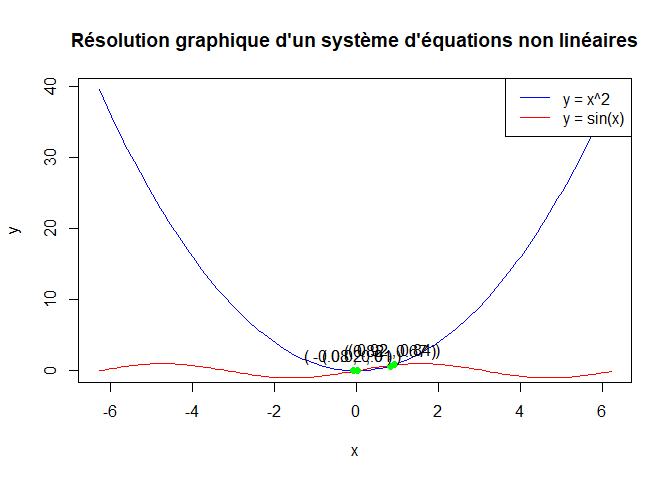
\includegraphics{PROJET_HEMA_files/figure-latex/unnamed-chunk-7-1.pdf}

\begin{Shaded}
\begin{Highlighting}[]
\CommentTok{\# Afficher les valeurs des solutions}
\FunctionTok{print}\NormalTok{(intersection\_points)}
\end{Highlighting}
\end{Shaded}

\begin{verbatim}
##             x            y
## 1 -0.08318531 0.0069197953
## 2  0.01681469 0.0002827339
## 3  0.81681469 0.6671862424
## 4  0.91681469 0.8405491810
\end{verbatim}

\hypertarget{exeemple-2}{%
\paragraph{Exeemple 2}\label{exeemple-2}}

\begin{Shaded}
\begin{Highlighting}[]
\CommentTok{\# Définition de la matrice des coefficients des équations}
\NormalTok{A }\OtherTok{=} \FunctionTok{matrix}\NormalTok{(}\DecValTok{0}\NormalTok{, }\DecValTok{2}\NormalTok{, }\DecValTok{3}\NormalTok{)  }\CommentTok{\# Crée une matrice 2x3 remplie de zéros}
\NormalTok{A[}\DecValTok{1}\NormalTok{,] }\OtherTok{=} \FunctionTok{c}\NormalTok{(}\DecValTok{2}\NormalTok{, }\DecValTok{2}\NormalTok{, }\DecValTok{3}\NormalTok{)   }\CommentTok{\# Coefficients de la première équation}
\NormalTok{A[}\DecValTok{2}\NormalTok{,] }\OtherTok{=} \FunctionTok{c}\NormalTok{(}\DecValTok{2}\NormalTok{, }\SpecialCharTok{{-}}\DecValTok{1}\NormalTok{, }\DecValTok{1}\NormalTok{)  }\CommentTok{\# Coefficients de la deuxième équation}

\CommentTok{\# Définition du vecteur des termes constants}
\NormalTok{B }\OtherTok{=} \FunctionTok{c}\NormalTok{(}\DecValTok{0}\NormalTok{, }\DecValTok{4}\NormalTok{)}

\CommentTok{\# Définition de la fonction de résolution du système}
\NormalTok{system }\OtherTok{=} \ControlFlowTok{function}\NormalTok{(z, A, B) \{}
  \CommentTok{\# Suppression des coefficients de z pour former une nouvelle matrice}
\NormalTok{  A2 }\OtherTok{=}\NormalTok{ A[,}\SpecialCharTok{{-}}\DecValTok{3}\NormalTok{]}
  \CommentTok{\# Calcul des termes constants ajustés en fonction de z}
\NormalTok{  B2 }\OtherTok{=}\NormalTok{ B }\SpecialCharTok{{-}}\NormalTok{ A[,}\DecValTok{3}\NormalTok{] }\SpecialCharTok{*}\NormalTok{ z}
  \CommentTok{\# Résolution du système et ajout de z à la solution}
\NormalTok{  res }\OtherTok{=} \FunctionTok{c}\NormalTok{(}\FunctionTok{solve}\NormalTok{(A2, B2), z)}
  \CommentTok{\# Renvoi du vecteur de solutions}
  \FunctionTok{return}\NormalTok{(res)}
\NormalTok{\}}

\CommentTok{\# Définition des valeurs de z pour lesquelles résoudre le système}
\NormalTok{Z }\OtherTok{=} \FunctionTok{matrix}\NormalTok{(}\FunctionTok{seq}\NormalTok{(}\SpecialCharTok{{-}}\DecValTok{20}\NormalTok{, }\DecValTok{20}\NormalTok{, }\AttributeTok{by =} \DecValTok{1}\NormalTok{), }\AttributeTok{ncol =} \DecValTok{1}\NormalTok{)}

\CommentTok{\# Application de la fonction système à chaque valeur de z et formatage des résultats}
\NormalTok{resultats }\OtherTok{=} \FunctionTok{apply}\NormalTok{(Z, }\AttributeTok{MARGIN =} \DecValTok{1}\NormalTok{, }\AttributeTok{FUN =}\NormalTok{ system, }\AttributeTok{A =}\NormalTok{ A, }\AttributeTok{B =}\NormalTok{ B)}
\NormalTok{resultats\_format }\OtherTok{=} \FunctionTok{as.matrix}\NormalTok{(}\FunctionTok{t}\NormalTok{(resultats), }\AttributeTok{dimnames =} \FunctionTok{list}\NormalTok{(}\ConstantTok{NULL}\NormalTok{, }\FunctionTok{c}\NormalTok{(}\StringTok{"x"}\NormalTok{, }\StringTok{"y"}\NormalTok{, }\StringTok{"z"}\NormalTok{)))}

\CommentTok{\# Affichage des résultats}
\NormalTok{resultats\_format}
\end{Highlighting}
\end{Shaded}

\begin{verbatim}
##              [,1]        [,2] [,3]
##  [1,]  18.0000000  12.0000000  -20
##  [2,]  17.1666667  11.3333333  -19
##  [3,]  16.3333333  10.6666667  -18
##  [4,]  15.5000000  10.0000000  -17
##  [5,]  14.6666667   9.3333333  -16
##  [6,]  13.8333333   8.6666667  -15
##  [7,]  13.0000000   8.0000000  -14
##  [8,]  12.1666667   7.3333333  -13
##  [9,]  11.3333333   6.6666667  -12
## [10,]  10.5000000   6.0000000  -11
## [11,]   9.6666667   5.3333333  -10
## [12,]   8.8333333   4.6666667   -9
## [13,]   8.0000000   4.0000000   -8
## [14,]   7.1666667   3.3333333   -7
## [15,]   6.3333333   2.6666667   -6
## [16,]   5.5000000   2.0000000   -5
## [17,]   4.6666667   1.3333333   -4
## [18,]   3.8333333   0.6666667   -3
## [19,]   3.0000000   0.0000000   -2
## [20,]   2.1666667  -0.6666667   -1
## [21,]   1.3333333  -1.3333333    0
## [22,]   0.5000000  -2.0000000    1
## [23,]  -0.3333333  -2.6666667    2
## [24,]  -1.1666667  -3.3333333    3
## [25,]  -2.0000000  -4.0000000    4
## [26,]  -2.8333333  -4.6666667    5
## [27,]  -3.6666667  -5.3333333    6
## [28,]  -4.5000000  -6.0000000    7
## [29,]  -5.3333333  -6.6666667    8
## [30,]  -6.1666667  -7.3333333    9
## [31,]  -7.0000000  -8.0000000   10
## [32,]  -7.8333333  -8.6666667   11
## [33,]  -8.6666667  -9.3333333   12
## [34,]  -9.5000000 -10.0000000   13
## [35,] -10.3333333 -10.6666667   14
## [36,] -11.1666667 -11.3333333   15
## [37,] -12.0000000 -12.0000000   16
## [38,] -12.8333333 -12.6666667   17
## [39,] -13.6666667 -13.3333333   18
## [40,] -14.5000000 -14.0000000   19
## [41,] -15.3333333 -14.6666667   20
\end{verbatim}

\begin{Shaded}
\begin{Highlighting}[]
\CommentTok{\# Résolution graphique \#\#\#\#\#\#\#\#\#\#\#\#\#\#\#\#\#\#\#\#\#\#\#\#\#\#\#\#\#\#\#\#\#\#\#\#\#\#\#\#\#\#\#\#\#\#}

\CommentTok{\# Définir les fonctions d\textquotesingle{}équations}
\NormalTok{equation1 }\OtherTok{\textless{}{-}} \ControlFlowTok{function}\NormalTok{(x) \{}
  \FunctionTok{return}\NormalTok{(x}\SpecialCharTok{\^{}}\DecValTok{2}\NormalTok{)}
\NormalTok{\}}

\NormalTok{equation2 }\OtherTok{\textless{}{-}} \ControlFlowTok{function}\NormalTok{(x) \{}
  \FunctionTok{return}\NormalTok{(}\FunctionTok{sin}\NormalTok{(x))}
\NormalTok{\}}

\CommentTok{\# Générer des valeurs de x pour le traçage}
\NormalTok{x }\OtherTok{\textless{}{-}} \FunctionTok{seq}\NormalTok{(}\SpecialCharTok{{-}}\DecValTok{2}\SpecialCharTok{*}\NormalTok{pi, }\DecValTok{2}\SpecialCharTok{*}\NormalTok{pi, }\AttributeTok{by =} \FloatTok{0.1}\NormalTok{)}

\CommentTok{\# Assuming x, equation1, and equation2 are defined}

\FunctionTok{library}\NormalTok{(ggplot2)}

\CommentTok{\# Create the ggplot2 object}

\FunctionTok{ggplot}\NormalTok{(}\AttributeTok{data =} \FunctionTok{data.frame}\NormalTok{(}\AttributeTok{x =}\NormalTok{ x), }\FunctionTok{aes}\NormalTok{(}\AttributeTok{x =}\NormalTok{ x)) }\SpecialCharTok{+}

  \CommentTok{\# Add the first curve (blue) with label}
  \FunctionTok{geom\_line}\NormalTok{(}\AttributeTok{y =} \FunctionTok{equation1}\NormalTok{(x), }\AttributeTok{col =} \StringTok{"blue"}\NormalTok{, }\AttributeTok{linetype =} \StringTok{"solid"}\NormalTok{, }\AttributeTok{label =} \StringTok{"Equation 1"}\NormalTok{) }\SpecialCharTok{+}

  \CommentTok{\# Add the second curve (red) with label}
  \FunctionTok{geom\_line}\NormalTok{(}\AttributeTok{y =} \FunctionTok{equation2}\NormalTok{(x), }\AttributeTok{col =} \StringTok{"red"}\NormalTok{, }\AttributeTok{linetype =} \StringTok{"dashed"}\NormalTok{, }\AttributeTok{label =} \StringTok{"Equation 2"}\NormalTok{) }\SpecialCharTok{+}

  \CommentTok{\# Add intersection points (assuming intersection\_points is a data frame)}
  \FunctionTok{geom\_point}\NormalTok{(}\AttributeTok{data =}\NormalTok{ intersection\_points, }\FunctionTok{aes}\NormalTok{(}\AttributeTok{x =}\NormalTok{ intersection\_points}\SpecialCharTok{$}\NormalTok{x, }\AttributeTok{y =}\NormalTok{ intersection\_points}\SpecialCharTok{$}\NormalTok{y), }
             \AttributeTok{col =} \StringTok{"blue"}\NormalTok{, }\AttributeTok{pch =} \DecValTok{16}\NormalTok{, }\AttributeTok{size =} \DecValTok{3}\NormalTok{) }\SpecialCharTok{+}  \CommentTok{\# Adjust size as needed}

  \CommentTok{\# Customize plot elements}
  \FunctionTok{labs}\NormalTok{(}\AttributeTok{x =} \StringTok{"x"}\NormalTok{, }\AttributeTok{y =} \StringTok{"y"}\NormalTok{) }\SpecialCharTok{+}
  \FunctionTok{ggtitle}\NormalTok{(}\StringTok{"Résolution graphique d\textquotesingle{}un système d\textquotesingle{}équations non linéaires"}\NormalTok{) }\SpecialCharTok{+}

  \CommentTok{\# Add the legend with updated syntax}
  \FunctionTok{scale\_linetype\_discrete}\NormalTok{(}\AttributeTok{name =} \StringTok{"Légende"}\NormalTok{) }\SpecialCharTok{+}
  \FunctionTok{guides}\NormalTok{(}\AttributeTok{linetype =} \FunctionTok{guide\_legend}\NormalTok{(}\AttributeTok{title.position =} \StringTok{"top"}\NormalTok{))  }\CommentTok{\# Legend positioning}
\end{Highlighting}
\end{Shaded}

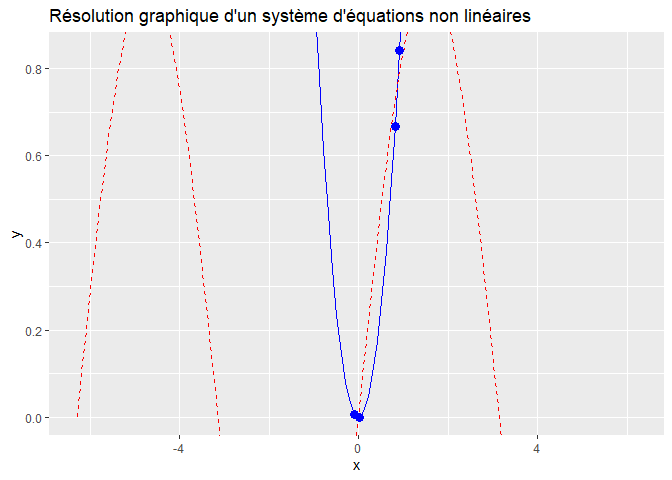
\includegraphics{PROJET_HEMA_files/figure-latex/unnamed-chunk-8-1.pdf}

\hypertarget{equations-linuxe9aires-ordinaire-classique-moduxe8le-de-lorenz}{%
\section{Equations Linéaires Ordinaire classique: Modèle de
Lorenz}\label{equations-linuxe9aires-ordinaire-classique-moduxe8le-de-lorenz}}

\hypertarget{da}{%
\subsubsection{Da}\label{da}}

\begin{Shaded}
\begin{Highlighting}[]
\NormalTok{model }\OtherTok{\textless{}{-}} \ControlFlowTok{function}\NormalTok{(t, Y, parameters) \{}
  \FunctionTok{with}\NormalTok{(}\FunctionTok{as.list}\NormalTok{(parameters), \{}
\NormalTok{    dy }\OtherTok{=} \SpecialCharTok{{-}}\NormalTok{a }\SpecialCharTok{*}\NormalTok{ Y}
    \FunctionTok{list}\NormalTok{(dy)}
\NormalTok{  \})}
\NormalTok{\}}

\CommentTok{\# On renseigne ensuite la jacobienne ∂y′∂y}

\NormalTok{jac }\OtherTok{\textless{}{-}} \ControlFlowTok{function}\NormalTok{(t, Y, parameters) \{}
  \FunctionTok{with}\NormalTok{(}\FunctionTok{as.list}\NormalTok{(parameters), \{}
\NormalTok{    PD[}\DecValTok{1}\NormalTok{, }\DecValTok{1}\NormalTok{] }\OtherTok{\textless{}{-}}\NormalTok{ a}
    \FunctionTok{return}\NormalTok{(PD)}
\NormalTok{  \})}
\NormalTok{\}}

\CommentTok{\# On peut ensuite résoudre l’EDO pour a=1 et y0=1 sur l’intervalle [0,1] des pas de temps de longeur 0.01}

\CommentTok{\#comme suit:}
\NormalTok{params }\OtherTok{\textless{}{-}} \FunctionTok{c}\NormalTok{(}\AttributeTok{a =} \DecValTok{1}\NormalTok{)}
\NormalTok{y0     }\OtherTok{\textless{}{-}} \FunctionTok{c}\NormalTok{(}\DecValTok{1}\NormalTok{)}
\NormalTok{times  }\OtherTok{\textless{}{-}} \FunctionTok{seq}\NormalTok{(}\DecValTok{0}\NormalTok{, }\DecValTok{1}\NormalTok{, }\AttributeTok{by =} \FloatTok{0.01}\NormalTok{)}
\NormalTok{PD     }\OtherTok{\textless{}{-}} \FunctionTok{matrix}\NormalTok{(}\DecValTok{0}\NormalTok{, }\AttributeTok{nrow =} \DecValTok{1}\NormalTok{, }\AttributeTok{ncol =} \DecValTok{1}\NormalTok{)}
\NormalTok{out\_atome }\OtherTok{\textless{}{-}} \FunctionTok{ode}\NormalTok{(y0, times, model, }\AttributeTok{parms =}\NormalTok{ params, }\AttributeTok{jacfun =}\NormalTok{ jac)}

\CommentTok{\# Le résultat est une matrice: {-} une colonne pour le temps (reprend les valeurs de times) {-} une colonne par dimension dans le système d’équationsdifférentielles}

\CommentTok{\#/*On peut vérifier que la solution numérique (en bleu) est confondue avec la solution analytique (en rouge)./*}

\NormalTok{plot\_data }\OtherTok{\textless{}{-}} \FunctionTok{data.frame}\NormalTok{(out\_atome) }\SpecialCharTok{\%\textgreater{}\%}
  \FunctionTok{mutate}\NormalTok{(}\AttributeTok{analytic =} \FunctionTok{exp}\NormalTok{(}\SpecialCharTok{{-}}\NormalTok{time)) }\SpecialCharTok{\%\textgreater{}\%}
  \FunctionTok{pivot\_longer}\NormalTok{(}\AttributeTok{cols =} \SpecialCharTok{{-}}\NormalTok{time,}
               \AttributeTok{names\_to =} \StringTok{"type"}\NormalTok{,}
               \AttributeTok{values\_to =} \StringTok{"value"}\NormalTok{)}
\FunctionTok{ggplot}\NormalTok{(plot\_data, }\FunctionTok{aes}\NormalTok{(}\AttributeTok{x =}\NormalTok{ time, }\AttributeTok{y =}\NormalTok{ value, }\AttributeTok{color =}\NormalTok{ type)) }\SpecialCharTok{+}
  \FunctionTok{geom\_line}\NormalTok{() }\SpecialCharTok{+}
  \FunctionTok{ylim}\NormalTok{(}\DecValTok{0}\NormalTok{, }\DecValTok{1}\NormalTok{) }\SpecialCharTok{+}
  \FunctionTok{theme}\NormalTok{(}\AttributeTok{legend.position =} \FunctionTok{c}\NormalTok{(}\FloatTok{0.95}\NormalTok{, }\FloatTok{0.95}\NormalTok{),}
        \AttributeTok{legend.justification =} \FunctionTok{c}\NormalTok{(}\DecValTok{1}\NormalTok{, }\DecValTok{1}\NormalTok{),}
        \AttributeTok{legend.background =} \FunctionTok{element\_rect}\NormalTok{(}\AttributeTok{fill =} \ConstantTok{NA}\NormalTok{))}
\end{Highlighting}
\end{Shaded}

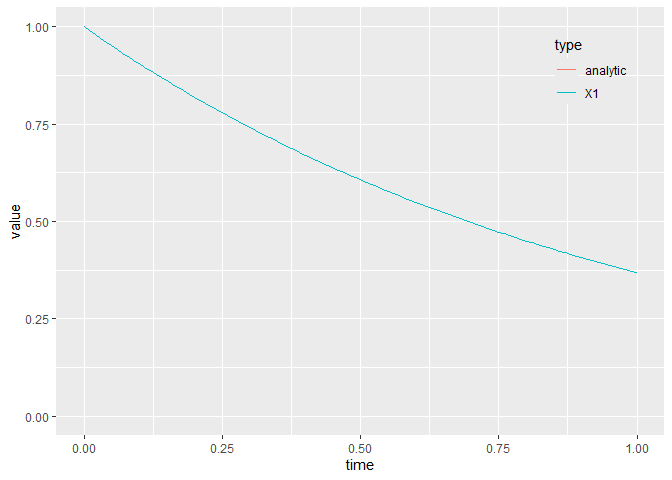
\includegraphics{PROJET_HEMA_files/figure-latex/unnamed-chunk-9-1.pdf}

\begin{Shaded}
\begin{Highlighting}[]
    \FunctionTok{diagnostics}\NormalTok{(out\_atome)}
\end{Highlighting}
\end{Shaded}

\begin{verbatim}
## 
## --------------------
## lsoda return code
## --------------------
## 
##   return code (idid) =  2 
##   Integration was successful.
## 
## --------------------
## INTEGER values
## --------------------
## 
##   1 The return code : 2 
##   2 The number of steps taken for the problem so far: 102 
##   3 The number of function evaluations for the problem so far: 133 
##   5 The method order last used (successfully): 6 
##   6 The order of the method to be attempted on the next step: 6 
##   7 If return flag =-4,-5: the largest component in error vector 0 
##   8 The length of the real work array actually required: 36 
##   9 The length of the integer work array actually required: 21 
##  14 The number of Jacobian evaluations and LU decompositions so far: 0 
##  15 The method indicator for the last succesful step,
##            1=adams (nonstiff), 2= bdf (stiff): 1 
##  16 The current method indicator to be attempted on the next step,
##            1=adams (nonstiff), 2= bdf (stiff): 1 
##  
## --------------------
## RSTATE values
## --------------------
## 
##   1 The step size in t last used (successfully): 0.01 
##   2 The step size to be attempted on the next step: 0.01 
##   3 The current value of the independent variable which the solver has reached: 1.00002 
##   4 Tolerance scale factor > 1.0 computed when requesting too much accuracy: 0 
##   5 The value of t at the time of the last method switch, if any: 0 
## 
\end{verbatim}

\hypertarget{exercice-1}{%
\subsection{Exercice 1}\label{exercice-1}}

\begin{Shaded}
\begin{Highlighting}[]
\CommentTok{\# Définir la fonction objective et les contraintes}
\NormalTok{obj }\OtherTok{\textless{}{-}} \FunctionTok{c}\NormalTok{(}\DecValTok{400}\NormalTok{, }\DecValTok{900}\NormalTok{, }\DecValTok{500}\NormalTok{, }\DecValTok{200}\NormalTok{)}
\NormalTok{mat }\OtherTok{\textless{}{-}} \FunctionTok{matrix}\NormalTok{(}\FunctionTok{c}\NormalTok{(}\DecValTok{40}\NormalTok{, }\DecValTok{75}\NormalTok{, }\DecValTok{30}\NormalTok{, }\DecValTok{15}\NormalTok{,   }\CommentTok{\# Contrainte 1}
                \SpecialCharTok{{-}}\DecValTok{30}\NormalTok{, }\SpecialCharTok{{-}}\DecValTok{40}\NormalTok{, }\SpecialCharTok{{-}}\DecValTok{20}\NormalTok{, }\SpecialCharTok{{-}}\DecValTok{10}\NormalTok{,   }\CommentTok{\# Contrainte 2}
                \DecValTok{40}\NormalTok{, }\DecValTok{75}\NormalTok{, }\DecValTok{0}\NormalTok{, }\DecValTok{0}\NormalTok{,   }\CommentTok{\# Contrainte 3}
                \SpecialCharTok{{-}}\DecValTok{1}\NormalTok{, }\DecValTok{0}\NormalTok{, }\DecValTok{0}\NormalTok{, }\DecValTok{0}\NormalTok{,   }\CommentTok{\# Contrainte 4}
                \DecValTok{0}\NormalTok{, }\SpecialCharTok{{-}}\DecValTok{1}\NormalTok{, }\DecValTok{0}\NormalTok{, }\DecValTok{0}\NormalTok{,   }\CommentTok{\# Contrainte 5}
                \DecValTok{0}\NormalTok{, }\DecValTok{0}\NormalTok{, }\DecValTok{1}\NormalTok{, }\DecValTok{0}\NormalTok{,   }\CommentTok{\# Contrainte 6}
                \DecValTok{0}\NormalTok{, }\DecValTok{0}\NormalTok{, }\SpecialCharTok{{-}}\DecValTok{1}\NormalTok{, }\DecValTok{0}\NormalTok{,  }\CommentTok{\# Contrainte 7}
                \DecValTok{0}\NormalTok{, }\DecValTok{0}\NormalTok{, }\DecValTok{0}\NormalTok{, }\DecValTok{1}\NormalTok{,   }\CommentTok{\# Contrainte 8}
                \DecValTok{0}\NormalTok{, }\DecValTok{0}\NormalTok{, }\DecValTok{0}\NormalTok{, }\SpecialCharTok{{-}}\DecValTok{1}\NormalTok{), }\CommentTok{\# Contrainte 9}
              \AttributeTok{nrow =} \DecValTok{9}\NormalTok{, }\AttributeTok{byrow =} \ConstantTok{TRUE}\NormalTok{)}
\NormalTok{dir }\OtherTok{\textless{}{-}} \FunctionTok{c}\NormalTok{(}\StringTok{"\textless{}="}\NormalTok{, }\StringTok{"\textgreater{}="}\NormalTok{, }\StringTok{"\textless{}="}\NormalTok{, }\StringTok{"\textgreater{}="}\NormalTok{, }\StringTok{"\textless{}="}\NormalTok{, }\StringTok{"\textless{}="}\NormalTok{, }\StringTok{"\textless{}="}\NormalTok{, }\StringTok{"\textgreater{}="}\NormalTok{, }\StringTok{"\textless{}="}\NormalTok{)}
\NormalTok{rhs }\OtherTok{\textless{}{-}} \FunctionTok{c}\NormalTok{(}\DecValTok{800}\NormalTok{, }\SpecialCharTok{{-}}\DecValTok{2000}\NormalTok{, }\DecValTok{500}\NormalTok{, }\SpecialCharTok{{-}}\DecValTok{3}\NormalTok{, }\SpecialCharTok{{-}}\DecValTok{2}\NormalTok{, }\DecValTok{10}\NormalTok{, }\SpecialCharTok{{-}}\DecValTok{5}\NormalTok{, }\DecValTok{10}\NormalTok{, }\SpecialCharTok{{-}}\DecValTok{5}\NormalTok{)}
\end{Highlighting}
\end{Shaded}

\hypertarget{ruxe9soudre-programme-linuxe9aire}{%
\subsubsection{Résoudre programme
linéaire}\label{ruxe9soudre-programme-linuxe9aire}}

\begin{Shaded}
\begin{Highlighting}[]
\NormalTok{result }\OtherTok{\textless{}{-}} \FunctionTok{lp}\NormalTok{(}\AttributeTok{direction =} \StringTok{"max"}\NormalTok{, }\AttributeTok{objective.in =}\NormalTok{ obj, }\AttributeTok{const.mat =}\NormalTok{ mat, }\AttributeTok{const.dir =}\NormalTok{ dir, }\AttributeTok{const.rhs =}\NormalTok{ rhs)}
\CommentTok{\# Afficher les quantités optimales}
\ControlFlowTok{if}\NormalTok{ (result}\SpecialCharTok{$}\NormalTok{status }\SpecialCharTok{==} \DecValTok{0}\NormalTok{) \{}
  \FunctionTok{print}\NormalTok{(}\FunctionTok{paste}\NormalTok{(}\StringTok{"x1 ="}\NormalTok{, result}\SpecialCharTok{$}\NormalTok{solution[}\DecValTok{1}\NormalTok{]))}
  \FunctionTok{print}\NormalTok{(}\FunctionTok{paste}\NormalTok{(}\StringTok{"x2 ="}\NormalTok{, result}\SpecialCharTok{$}\NormalTok{solution[}\DecValTok{2}\NormalTok{]))}
  \FunctionTok{print}\NormalTok{(}\FunctionTok{paste}\NormalTok{(}\StringTok{"x3 ="}\NormalTok{, result}\SpecialCharTok{$}\NormalTok{solution[}\DecValTok{3}\NormalTok{]))}
  \FunctionTok{print}\NormalTok{(}\FunctionTok{paste}\NormalTok{(}\StringTok{"x4 ="}\NormalTok{, result}\SpecialCharTok{$}\NormalTok{solution[}\DecValTok{4}\NormalTok{]))}
\NormalTok{\} }\ControlFlowTok{else}\NormalTok{ \{}
  \FunctionTok{print}\NormalTok{(}\StringTok{"Aucune solution optimale trouvée."}\NormalTok{)}
\NormalTok{\}}
\end{Highlighting}
\end{Shaded}

\begin{verbatim}
## [1] "x1 = 0"
## [1] "x2 = 2"
## [1] "x3 = 10"
## [1] "x4 = 23.3333333333333"
\end{verbatim}

\begin{Shaded}
\begin{Highlighting}[]
\CommentTok{\# Afficher les résultats}
\FunctionTok{print}\NormalTok{(result)}
\end{Highlighting}
\end{Shaded}

\begin{verbatim}
## Success: the objective function is 11466.67
\end{verbatim}

\hypertarget{exercice-2}{%
\section{Exercice 2}\label{exercice-2}}

\hypertarget{la-ruxe9partition-uxe9quitable-des-budgets-entre-les-secteurs-cluxe9s-dans-les-pays-de-lafrique-de-louest}{%
\subsubsection{La répartition équitable des budgets entre les secteurs
clés dans les pays de l'Afrique de
l'Ouest}\label{la-ruxe9partition-uxe9quitable-des-budgets-entre-les-secteurs-cluxe9s-dans-les-pays-de-lafrique-de-louest}}

\begin{Shaded}
\begin{Highlighting}[]
\CommentTok{\# Données pour les pays de l\textquotesingle{}Afrique de l\textquotesingle{}Ouest}
\NormalTok{pays }\OtherTok{\textless{}{-}} \FunctionTok{c}\NormalTok{(}\StringTok{"Bénin"}\NormalTok{, }\StringTok{"Burkina Faso"}\NormalTok{, }\StringTok{"Cap{-}Vert"}\NormalTok{, }\StringTok{"Côte d\textquotesingle{}Ivoire"}\NormalTok{, }\StringTok{"Gambie"}\NormalTok{, }\StringTok{"Ghana"}\NormalTok{, }\StringTok{"Guinée"}\NormalTok{, }\StringTok{"Guinée{-}Bissau"}\NormalTok{, }\StringTok{"Liberia"}\NormalTok{, }\StringTok{"Mali"}\NormalTok{, }\StringTok{"Niger"}\NormalTok{, }\StringTok{"Nigeria"}\NormalTok{, }\StringTok{"Sénégal"}\NormalTok{, }\StringTok{"Sierra Leone"}\NormalTok{, }\StringTok{"Togo"}\NormalTok{)}
\NormalTok{budget }\OtherTok{\textless{}{-}} \FunctionTok{c}\NormalTok{(}\DecValTok{1000}\NormalTok{, }\DecValTok{1200}\NormalTok{, }\DecValTok{1100}\NormalTok{, }\DecValTok{1300}\NormalTok{, }\DecValTok{900}\NormalTok{, }\DecValTok{1400}\NormalTok{, }\DecValTok{1500}\NormalTok{, }\DecValTok{1600}\NormalTok{, }\DecValTok{1700}\NormalTok{, }\DecValTok{1800}\NormalTok{, }\DecValTok{1900}\NormalTok{, }\DecValTok{2000}\NormalTok{, }\DecValTok{2100}\NormalTok{, }\DecValTok{2200}\NormalTok{, }\DecValTok{2300}\NormalTok{) }\CommentTok{\# Budgets spécifiques pour chaque pays}
\CommentTok{\# Secteurs clés et poids}
\NormalTok{secteurs }\OtherTok{\textless{}{-}} \FunctionTok{c}\NormalTok{(}\StringTok{"Education"}\NormalTok{, }\StringTok{"Santé"}\NormalTok{, }\StringTok{"Armée"}\NormalTok{, }\StringTok{"Infrastructures"}\NormalTok{)}
\NormalTok{poids }\OtherTok{\textless{}{-}} \FunctionTok{c}\NormalTok{(}\FloatTok{0.3}\NormalTok{, }\FloatTok{0.3}\NormalTok{, }\FloatTok{0.2}\NormalTok{, }\FloatTok{0.2}\NormalTok{) }\CommentTok{\# Poids pour chaque secteur}

\CommentTok{\# Création du dataframe}
\NormalTok{data }\OtherTok{\textless{}{-}} \FunctionTok{data.frame}\NormalTok{(}\AttributeTok{Pays =}\NormalTok{ pays, budget , }\AttributeTok{Education =} \DecValTok{0}\NormalTok{, Santé }\OtherTok{=} \DecValTok{0}\NormalTok{, Armée }\OtherTok{=} \DecValTok{0}\NormalTok{, }\AttributeTok{Infrastructures =} \DecValTok{0}\NormalTok{)}
\FunctionTok{print}\NormalTok{(data)}
\end{Highlighting}
\end{Shaded}

\begin{verbatim}
##             Pays budget Education Santé Armée Infrastructures
## 1          Bénin   1000         0     0     0               0
## 2   Burkina Faso   1200         0     0     0               0
## 3       Cap-Vert   1100         0     0     0               0
## 4  Côte d'Ivoire   1300         0     0     0               0
## 5         Gambie    900         0     0     0               0
## 6          Ghana   1400         0     0     0               0
## 7         Guinée   1500         0     0     0               0
## 8  Guinée-Bissau   1600         0     0     0               0
## 9        Liberia   1700         0     0     0               0
## 10          Mali   1800         0     0     0               0
## 11         Niger   1900         0     0     0               0
## 12       Nigeria   2000         0     0     0               0
## 13       Sénégal   2100         0     0     0               0
## 14  Sierra Leone   2200         0     0     0               0
## 15          Togo   2300         0     0     0               0
\end{verbatim}

\hypertarget{effectuons-la-repartition-optimale-des-budgets-en-fonction-des-secteurs-stratuxe9giques}{%
\subsubsection{Effectuons la repartition optimale des Budgets en
fonction des Secteurs
stratégiques}\label{effectuons-la-repartition-optimale-des-budgets-en-fonction-des-secteurs-stratuxe9giques}}

\begin{Shaded}
\begin{Highlighting}[]
\CommentTok{\# base de données }
\NormalTok{pays }\OtherTok{\textless{}{-}} \FunctionTok{c}\NormalTok{(}\StringTok{"Bénin"}\NormalTok{, }\StringTok{"Burkina Faso"}\NormalTok{, }\StringTok{"Cap{-}Vert"}\NormalTok{, }\StringTok{"Côte d\textquotesingle{}Ivoire"}\NormalTok{, }\StringTok{"Gambie"}\NormalTok{, }\StringTok{"Ghana"}\NormalTok{, }\StringTok{"Guinée"}\NormalTok{, }\StringTok{"Guinée{-}Bissau"}\NormalTok{, }\StringTok{"Liberia"}\NormalTok{, }\StringTok{"Mali"}\NormalTok{, }\StringTok{"Niger"}\NormalTok{, }\StringTok{"Nigeria"}\NormalTok{, }\StringTok{"Sénégal"}\NormalTok{, }\StringTok{"Sierra Leone"}\NormalTok{, }\StringTok{"Togo"}\NormalTok{)}
\NormalTok{budget }\OtherTok{\textless{}{-}} \FunctionTok{c}\NormalTok{(}\DecValTok{1000}\NormalTok{, }\DecValTok{1200}\NormalTok{, }\DecValTok{1100}\NormalTok{, }\DecValTok{1300}\NormalTok{, }\DecValTok{900}\NormalTok{, }\DecValTok{1400}\NormalTok{, }\DecValTok{1500}\NormalTok{, }\DecValTok{1600}\NormalTok{, }\DecValTok{1700}\NormalTok{, }\DecValTok{1800}\NormalTok{, }\DecValTok{1900}\NormalTok{, }\DecValTok{2000}\NormalTok{, }\DecValTok{2100}\NormalTok{, }\DecValTok{2200}\NormalTok{, }\DecValTok{2300}\NormalTok{) }\CommentTok{\# Budgets spécifiques pour chaque pays}

\CommentTok{\# Générer des allocations sectorielles fixes pour chaque pays}
\NormalTok{poid\_agriculture }\OtherTok{\textless{}{-}} \FunctionTok{c}\NormalTok{(}\DecValTok{400}\NormalTok{, }\DecValTok{450}\NormalTok{, }\DecValTok{350}\NormalTok{, }\DecValTok{500}\NormalTok{, }\DecValTok{300}\NormalTok{, }\DecValTok{450}\NormalTok{, }\DecValTok{400}\NormalTok{, }\DecValTok{350}\NormalTok{, }\DecValTok{500}\NormalTok{, }\DecValTok{450}\NormalTok{, }\DecValTok{400}\NormalTok{, }\DecValTok{500}\NormalTok{, }\DecValTok{450}\NormalTok{, }\DecValTok{400}\NormalTok{, }\DecValTok{350}\NormalTok{)}
\NormalTok{poid\_industrie }\OtherTok{\textless{}{-}} \FunctionTok{c}\NormalTok{(}\DecValTok{400}\NormalTok{, }\DecValTok{450}\NormalTok{, }\DecValTok{350}\NormalTok{, }\DecValTok{500}\NormalTok{, }\DecValTok{300}\NormalTok{, }\DecValTok{450}\NormalTok{, }\DecValTok{400}\NormalTok{, }\DecValTok{350}\NormalTok{, }\DecValTok{500}\NormalTok{, }\DecValTok{450}\NormalTok{, }\DecValTok{400}\NormalTok{, }\DecValTok{500}\NormalTok{, }\DecValTok{450}\NormalTok{, }\DecValTok{400}\NormalTok{, }\DecValTok{350}\NormalTok{)}
\NormalTok{poid\_education }\OtherTok{\textless{}{-}} \FunctionTok{c}\NormalTok{(}\DecValTok{300}\NormalTok{, }\DecValTok{350}\NormalTok{, }\DecValTok{250}\NormalTok{, }\DecValTok{400}\NormalTok{, }\DecValTok{200}\NormalTok{, }\DecValTok{350}\NormalTok{, }\DecValTok{300}\NormalTok{, }\DecValTok{250}\NormalTok{, }\DecValTok{400}\NormalTok{, }\DecValTok{350}\NormalTok{, }\DecValTok{300}\NormalTok{, }\DecValTok{400}\NormalTok{, }\DecValTok{350}\NormalTok{, }\DecValTok{300}\NormalTok{, }\DecValTok{250}\NormalTok{)}
\NormalTok{poid\_sante }\OtherTok{\textless{}{-}} \FunctionTok{c}\NormalTok{(}\DecValTok{75}\NormalTok{, }\DecValTok{85}\NormalTok{, }\DecValTok{65}\NormalTok{, }\DecValTok{95}\NormalTok{, }\DecValTok{55}\NormalTok{, }\DecValTok{85}\NormalTok{, }\DecValTok{75}\NormalTok{, }\DecValTok{65}\NormalTok{, }\DecValTok{95}\NormalTok{, }\DecValTok{85}\NormalTok{, }\DecValTok{75}\NormalTok{, }\DecValTok{95}\NormalTok{, }\DecValTok{85}\NormalTok{, }\DecValTok{75}\NormalTok{, }\DecValTok{65}\NormalTok{)}
\NormalTok{poid\_infrastructure }\OtherTok{\textless{}{-}} \FunctionTok{c}\NormalTok{(}\DecValTok{35}\NormalTok{, }\DecValTok{40}\NormalTok{, }\DecValTok{30}\NormalTok{, }\DecValTok{45}\NormalTok{, }\DecValTok{25}\NormalTok{, }\DecValTok{40}\NormalTok{, }\DecValTok{35}\NormalTok{, }\DecValTok{30}\NormalTok{, }\DecValTok{45}\NormalTok{, }\DecValTok{40}\NormalTok{, }\DecValTok{35}\NormalTok{, }\DecValTok{45}\NormalTok{, }\DecValTok{40}\NormalTok{, }\DecValTok{35}\NormalTok{, }\DecValTok{30}\NormalTok{)}
\NormalTok{poid\_recherche }\OtherTok{\textless{}{-}} \FunctionTok{c}\NormalTok{(}\DecValTok{50}\NormalTok{, }\DecValTok{60}\NormalTok{, }\DecValTok{40}\NormalTok{, }\DecValTok{70}\NormalTok{, }\DecValTok{30}\NormalTok{, }\DecValTok{60}\NormalTok{, }\DecValTok{50}\NormalTok{, }\DecValTok{40}\NormalTok{, }\DecValTok{70}\NormalTok{, }\DecValTok{60}\NormalTok{, }\DecValTok{50}\NormalTok{, }\DecValTok{70}\NormalTok{, }\DecValTok{60}\NormalTok{, }\DecValTok{50}\NormalTok{, }\DecValTok{40}\NormalTok{)}

\NormalTok{data }\OtherTok{\textless{}{-}} \FunctionTok{data.frame}\NormalTok{(pays, budget, poid\_agriculture, poid\_industrie, poid\_education, poid\_sante, poid\_infrastructure, poid\_recherche)}


\CommentTok{\# Début de la boucle}
\ControlFlowTok{for}\NormalTok{ (i }\ControlFlowTok{in} \DecValTok{1}\SpecialCharTok{:}\FunctionTok{nrow}\NormalTok{(data)) \{}
  \CommentTok{\# Extraire les valeurs nécessaires pour l\textquotesingle{}itération i}
\NormalTok{  budget }\OtherTok{\textless{}{-}}\NormalTok{ data}\SpecialCharTok{$}\NormalTok{budget[i]}
\NormalTok{  agriculture }\OtherTok{\textless{}{-}}\NormalTok{ data}\SpecialCharTok{$}\NormalTok{poid\_agriculture[i]}
\NormalTok{  industrie }\OtherTok{\textless{}{-}}\NormalTok{ data}\SpecialCharTok{$}\NormalTok{poid\_industrie[i]}
\NormalTok{  education }\OtherTok{\textless{}{-}}\NormalTok{ data}\SpecialCharTok{$}\NormalTok{poid\_education[i]}
\NormalTok{  sante }\OtherTok{\textless{}{-}}\NormalTok{ data}\SpecialCharTok{$}\NormalTok{poid\_sante[i]}
\NormalTok{  infrastructure }\OtherTok{\textless{}{-}}\NormalTok{ data}\SpecialCharTok{$}\NormalTok{poid\_infrastructure[i]}
  
  \CommentTok{\# Définir la fonction du solveur}
\NormalTok{  mysolver }\OtherTok{\textless{}{-}} \ControlFlowTok{function}\NormalTok{(p) \{}
\NormalTok{    a }\OtherTok{\textless{}{-}}\NormalTok{ p[}\DecValTok{1}\NormalTok{]}
\NormalTok{    b }\OtherTok{\textless{}{-}}\NormalTok{ p[}\DecValTok{2}\NormalTok{]}
\NormalTok{    c }\OtherTok{\textless{}{-}}\NormalTok{ p[}\DecValTok{3}\NormalTok{]}
\NormalTok{    d }\OtherTok{\textless{}{-}}\NormalTok{ p[}\DecValTok{4}\NormalTok{]}
\NormalTok{    e }\OtherTok{\textless{}{-}}\NormalTok{ p[}\DecValTok{5}\NormalTok{]}
\NormalTok{    lnf}\OtherTok{\textless{}{-}} \FunctionTok{numeric}\NormalTok{(}\DecValTok{5}\NormalTok{)}
\NormalTok{    lnf[}\DecValTok{1}\NormalTok{] }\OtherTok{\textless{}{-}}\NormalTok{ ((a}\SpecialCharTok{*}\NormalTok{agriculture}\SpecialCharTok{/}\NormalTok{budget)}\SpecialCharTok{/}\NormalTok{(a}\SpecialCharTok{*}\NormalTok{agriculture}\SpecialCharTok{/}\NormalTok{budget }\SpecialCharTok{+}\NormalTok{ b}\SpecialCharTok{*}\NormalTok{industrie}\SpecialCharTok{/}\NormalTok{budget }\SpecialCharTok{+}\NormalTok{ c}\SpecialCharTok{*}\NormalTok{education}\SpecialCharTok{/}\NormalTok{budget }\SpecialCharTok{+}\NormalTok{ d}\SpecialCharTok{*}\NormalTok{sante}\SpecialCharTok{/}\NormalTok{budget }\SpecialCharTok{+}\NormalTok{ e}\SpecialCharTok{*}\NormalTok{infrastructure}\SpecialCharTok{/}\NormalTok{budget) }\SpecialCharTok{{-}} \DecValTok{1}\SpecialCharTok{/}\DecValTok{5}\NormalTok{)}
\NormalTok{    lnf[}\DecValTok{2}\NormalTok{] }\OtherTok{\textless{}{-}}\NormalTok{ ((b}\SpecialCharTok{*}\NormalTok{industrie}\SpecialCharTok{/}\NormalTok{budget)}\SpecialCharTok{/}\NormalTok{(a}\SpecialCharTok{*}\NormalTok{agriculture}\SpecialCharTok{/}\NormalTok{budget }\SpecialCharTok{+}\NormalTok{ b}\SpecialCharTok{*}\NormalTok{industrie}\SpecialCharTok{/}\NormalTok{budget }\SpecialCharTok{+}\NormalTok{ c}\SpecialCharTok{*}\NormalTok{education}\SpecialCharTok{/}\NormalTok{budget }\SpecialCharTok{+}\NormalTok{ d}\SpecialCharTok{*}\NormalTok{sante}\SpecialCharTok{/}\NormalTok{budget }\SpecialCharTok{+}\NormalTok{ e}\SpecialCharTok{*}\NormalTok{infrastructure}\SpecialCharTok{/}\NormalTok{budget) }\SpecialCharTok{{-}} \DecValTok{1}\SpecialCharTok{/}\DecValTok{5}\NormalTok{)}
\NormalTok{    lnf[}\DecValTok{3}\NormalTok{] }\OtherTok{\textless{}{-}}\NormalTok{ ((c}\SpecialCharTok{*}\NormalTok{education}\SpecialCharTok{/}\NormalTok{budget)}\SpecialCharTok{/}\NormalTok{(a}\SpecialCharTok{*}\NormalTok{agriculture}\SpecialCharTok{/}\NormalTok{budget }\SpecialCharTok{+}\NormalTok{ b}\SpecialCharTok{*}\NormalTok{industrie}\SpecialCharTok{/}\NormalTok{budget }\SpecialCharTok{+}\NormalTok{ c}\SpecialCharTok{*}\NormalTok{education}\SpecialCharTok{/}\NormalTok{budget }\SpecialCharTok{+}\NormalTok{ d}\SpecialCharTok{*}\NormalTok{sante}\SpecialCharTok{/}\NormalTok{budget }\SpecialCharTok{+}\NormalTok{ e}\SpecialCharTok{*}\NormalTok{infrastructure}\SpecialCharTok{/}\NormalTok{budget) }\SpecialCharTok{{-}} \DecValTok{1}\SpecialCharTok{/}\DecValTok{5}\NormalTok{)}
\NormalTok{    lnf[}\DecValTok{4}\NormalTok{] }\OtherTok{\textless{}{-}}\NormalTok{ ((d}\SpecialCharTok{*}\NormalTok{sante}\SpecialCharTok{/}\NormalTok{budget)}\SpecialCharTok{/}\NormalTok{(a}\SpecialCharTok{*}\NormalTok{agriculture}\SpecialCharTok{/}\NormalTok{budget }\SpecialCharTok{+}\NormalTok{ b}\SpecialCharTok{*}\NormalTok{industrie}\SpecialCharTok{/}\NormalTok{budget }\SpecialCharTok{+}\NormalTok{ c}\SpecialCharTok{*}\NormalTok{education}\SpecialCharTok{/}\NormalTok{budget }\SpecialCharTok{+}\NormalTok{ d}\SpecialCharTok{*}\NormalTok{sante}\SpecialCharTok{/}\NormalTok{budget }\SpecialCharTok{+}\NormalTok{ e}\SpecialCharTok{*}\NormalTok{infrastructure}\SpecialCharTok{/}\NormalTok{budget) }\SpecialCharTok{{-}} \DecValTok{1}\SpecialCharTok{/}\DecValTok{5}\NormalTok{)}
\NormalTok{    lnf[}\DecValTok{5}\NormalTok{] }\OtherTok{\textless{}{-}}\NormalTok{ (a }\SpecialCharTok{+}\NormalTok{ b }\SpecialCharTok{+}\NormalTok{ c }\SpecialCharTok{+}\NormalTok{ d }\SpecialCharTok{+}\NormalTok{ e }\SpecialCharTok{{-}}\NormalTok{ budget)}
    \FunctionTok{return}\NormalTok{(lnf)}
\NormalTok{  \}}
  
  \CommentTok{\# Appeler le solveur}
\NormalTok{  result }\OtherTok{\textless{}{-}}\NormalTok{ nleqslv}\SpecialCharTok{::}\FunctionTok{nleqslv}\NormalTok{( }\FunctionTok{c}\NormalTok{(}\DecValTok{1}\NormalTok{, }\DecValTok{1}\NormalTok{, }\DecValTok{1}\NormalTok{, }\DecValTok{1}\NormalTok{, }\DecValTok{1}\NormalTok{), mysolver, }\AttributeTok{method =} \StringTok{"Broyden"}\NormalTok{,}\AttributeTok{control =} \FunctionTok{list}\NormalTok{( }\AttributeTok{xtol=} \FloatTok{1e{-}8}\NormalTok{,}\AttributeTok{ftol=}\FloatTok{1e{-}15}\NormalTok{) )}
\NormalTok{  p }\OtherTok{\textless{}{-}}\NormalTok{ result}\SpecialCharTok{$}\NormalTok{x}
  
  \CommentTok{\# Assigner les résultats aux variables allocation\_agriculture, allocation\_industrie, allocation\_education, allocation\_sante}
\NormalTok{  data}\SpecialCharTok{$}\NormalTok{allocation\_agriculture[i] }\OtherTok{\textless{}{-}}\NormalTok{ p[}\DecValTok{1}\NormalTok{]}
\NormalTok{  data}\SpecialCharTok{$}\NormalTok{allocation\_industrie[i] }\OtherTok{\textless{}{-}}\NormalTok{ p[}\DecValTok{2}\NormalTok{]}
\NormalTok{  data}\SpecialCharTok{$}\NormalTok{allocation\_education[i] }\OtherTok{\textless{}{-}}\NormalTok{ p[}\DecValTok{3}\NormalTok{]}
\NormalTok{  data}\SpecialCharTok{$}\NormalTok{allocation\_sante[i] }\OtherTok{\textless{}{-}}\NormalTok{ p[}\DecValTok{4}\NormalTok{]}
\NormalTok{  data}\SpecialCharTok{$}\NormalTok{allocation\_infrastructure[i] }\OtherTok{\textless{}{-}}\NormalTok{ p[}\DecValTok{5}\NormalTok{]}
\NormalTok{\}}

\CommentTok{\#View(data)}



\CommentTok{\# Installer et charger les packages nécessaires}
\ControlFlowTok{if}\NormalTok{ (}\SpecialCharTok{!}\FunctionTok{require}\NormalTok{(stats)) }\FunctionTok{install.packages}\NormalTok{(}\StringTok{"stats"}\NormalTok{)}
\FunctionTok{library}\NormalTok{(stats)}

\CommentTok{\# Générer une base de données fictive}
\CommentTok{\# (les données restent les mêmes)}

\CommentTok{\# Créer les variables allocation\_agriculture, allocation\_industrie, allocation\_education, allocation\_sante, allocation\_infrastructure initialisées à 0}
\NormalTok{data}\SpecialCharTok{$}\NormalTok{allocation\_agriculture }\OtherTok{\textless{}{-}} \DecValTok{0}
\NormalTok{data}\SpecialCharTok{$}\NormalTok{allocation\_industrie }\OtherTok{\textless{}{-}} \DecValTok{0}
\NormalTok{data}\SpecialCharTok{$}\NormalTok{allocation\_education }\OtherTok{\textless{}{-}} \DecValTok{0}
\NormalTok{data}\SpecialCharTok{$}\NormalTok{allocation\_sante }\OtherTok{\textless{}{-}} \DecValTok{0}
\NormalTok{data}\SpecialCharTok{$}\NormalTok{allocation\_infrastructure }\OtherTok{\textless{}{-}} \DecValTok{0}

\CommentTok{\# Début de la boucle}
\ControlFlowTok{for}\NormalTok{ (i }\ControlFlowTok{in} \DecValTok{1}\SpecialCharTok{:}\FunctionTok{nrow}\NormalTok{(data)) \{}
  \CommentTok{\# Extraire les valeurs nécessaires pour l\textquotesingle{}itération i}
\NormalTok{  budget }\OtherTok{\textless{}{-}}\NormalTok{ data}\SpecialCharTok{$}\NormalTok{budget[i]}
\NormalTok{  agriculture }\OtherTok{\textless{}{-}}\NormalTok{ data}\SpecialCharTok{$}\NormalTok{poid\_agriculture[i]}
\NormalTok{  industrie }\OtherTok{\textless{}{-}}\NormalTok{ data}\SpecialCharTok{$}\NormalTok{poid\_industrie[i]}
\NormalTok{  education }\OtherTok{\textless{}{-}}\NormalTok{ data}\SpecialCharTok{$}\NormalTok{poid\_education[i]}
\NormalTok{  sante }\OtherTok{\textless{}{-}}\NormalTok{ data}\SpecialCharTok{$}\NormalTok{poid\_sante[i]}
\NormalTok{  infrastructure }\OtherTok{\textless{}{-}}\NormalTok{ data}\SpecialCharTok{$}\NormalTok{poid\_infrastructure[i]}
  
  \CommentTok{\# Définir la fonction du solveur}
\NormalTok{  mysolver }\OtherTok{\textless{}{-}} \ControlFlowTok{function}\NormalTok{(p) \{}
\NormalTok{    a }\OtherTok{\textless{}{-}}\NormalTok{ p[}\DecValTok{1}\NormalTok{]}
\NormalTok{    b }\OtherTok{\textless{}{-}}\NormalTok{ p[}\DecValTok{2}\NormalTok{]}
\NormalTok{    c }\OtherTok{\textless{}{-}}\NormalTok{ p[}\DecValTok{3}\NormalTok{]}
\NormalTok{    d }\OtherTok{\textless{}{-}}\NormalTok{ p[}\DecValTok{4}\NormalTok{]}
\NormalTok{    e }\OtherTok{\textless{}{-}}\NormalTok{ p[}\DecValTok{5}\NormalTok{]}
\NormalTok{    lnf}\OtherTok{\textless{}{-}} \FunctionTok{numeric}\NormalTok{(}\DecValTok{5}\NormalTok{)}
\NormalTok{    lnf[}\DecValTok{1}\NormalTok{] }\OtherTok{\textless{}{-}}\NormalTok{ ((a}\SpecialCharTok{*}\NormalTok{agriculture}\SpecialCharTok{/}\NormalTok{budget)}\SpecialCharTok{/}\NormalTok{(a}\SpecialCharTok{*}\NormalTok{agriculture}\SpecialCharTok{/}\NormalTok{budget }\SpecialCharTok{+}\NormalTok{ b}\SpecialCharTok{*}\NormalTok{industrie}\SpecialCharTok{/}\NormalTok{budget }\SpecialCharTok{+}\NormalTok{ c}\SpecialCharTok{*}\NormalTok{education}\SpecialCharTok{/}\NormalTok{budget }\SpecialCharTok{+}\NormalTok{ d}\SpecialCharTok{*}\NormalTok{sante}\SpecialCharTok{/}\NormalTok{budget }\SpecialCharTok{+}\NormalTok{ e}\SpecialCharTok{*}\NormalTok{infrastructure}\SpecialCharTok{/}\NormalTok{budget) }\SpecialCharTok{{-}} \DecValTok{1}\SpecialCharTok{/}\DecValTok{5}\NormalTok{)}
\NormalTok{    lnf[}\DecValTok{2}\NormalTok{] }\OtherTok{\textless{}{-}}\NormalTok{ ((b}\SpecialCharTok{*}\NormalTok{industrie}\SpecialCharTok{/}\NormalTok{budget)}\SpecialCharTok{/}\NormalTok{(a}\SpecialCharTok{*}\NormalTok{agriculture}\SpecialCharTok{/}\NormalTok{budget }\SpecialCharTok{+}\NormalTok{ b}\SpecialCharTok{*}\NormalTok{industrie}\SpecialCharTok{/}\NormalTok{budget }\SpecialCharTok{+}\NormalTok{ c}\SpecialCharTok{*}\NormalTok{education}\SpecialCharTok{/}\NormalTok{budget }\SpecialCharTok{+}\NormalTok{ d}\SpecialCharTok{*}\NormalTok{sante}\SpecialCharTok{/}\NormalTok{budget }\SpecialCharTok{+}\NormalTok{ e}\SpecialCharTok{*}\NormalTok{infrastructure}\SpecialCharTok{/}\NormalTok{budget) }\SpecialCharTok{{-}} \DecValTok{1}\SpecialCharTok{/}\DecValTok{5}\NormalTok{)}
\NormalTok{    lnf[}\DecValTok{3}\NormalTok{] }\OtherTok{\textless{}{-}}\NormalTok{ ((c}\SpecialCharTok{*}\NormalTok{education}\SpecialCharTok{/}\NormalTok{budget)}\SpecialCharTok{/}\NormalTok{(a}\SpecialCharTok{*}\NormalTok{agriculture}\SpecialCharTok{/}\NormalTok{budget }\SpecialCharTok{+}\NormalTok{ b}\SpecialCharTok{*}\NormalTok{industrie}\SpecialCharTok{/}\NormalTok{budget }\SpecialCharTok{+}\NormalTok{ c}\SpecialCharTok{*}\NormalTok{education}\SpecialCharTok{/}\NormalTok{budget }\SpecialCharTok{+}\NormalTok{ d}\SpecialCharTok{*}\NormalTok{sante}\SpecialCharTok{/}\NormalTok{budget }\SpecialCharTok{+}\NormalTok{ e}\SpecialCharTok{*}\NormalTok{infrastructure}\SpecialCharTok{/}\NormalTok{budget) }\SpecialCharTok{{-}} \DecValTok{1}\SpecialCharTok{/}\DecValTok{5}\NormalTok{)}
\NormalTok{    lnf[}\DecValTok{4}\NormalTok{] }\OtherTok{\textless{}{-}}\NormalTok{ ((d}\SpecialCharTok{*}\NormalTok{sante}\SpecialCharTok{/}\NormalTok{budget)}\SpecialCharTok{/}\NormalTok{(a}\SpecialCharTok{*}\NormalTok{agriculture}\SpecialCharTok{/}\NormalTok{budget }\SpecialCharTok{+}\NormalTok{ b}\SpecialCharTok{*}\NormalTok{industrie}\SpecialCharTok{/}\NormalTok{budget }\SpecialCharTok{+}\NormalTok{ c}\SpecialCharTok{*}\NormalTok{education}\SpecialCharTok{/}\NormalTok{budget }\SpecialCharTok{+}\NormalTok{ d}\SpecialCharTok{*}\NormalTok{sante}\SpecialCharTok{/}\NormalTok{budget }\SpecialCharTok{+}\NormalTok{ e}\SpecialCharTok{*}\NormalTok{infrastructure}\SpecialCharTok{/}\NormalTok{budget) }\SpecialCharTok{{-}} \DecValTok{1}\SpecialCharTok{/}\DecValTok{5}\NormalTok{)}
\NormalTok{    lnf[}\DecValTok{5}\NormalTok{] }\OtherTok{\textless{}{-}}\NormalTok{ (a }\SpecialCharTok{+}\NormalTok{ b }\SpecialCharTok{+}\NormalTok{ c }\SpecialCharTok{+}\NormalTok{ d }\SpecialCharTok{+}\NormalTok{ e }\SpecialCharTok{{-}}\NormalTok{ budget)}
    \FunctionTok{return}\NormalTok{(}\FunctionTok{sum}\NormalTok{(lnf}\SpecialCharTok{\^{}}\DecValTok{2}\NormalTok{))}
\NormalTok{  \}}
  
  \CommentTok{\# Appeler le solveur}
\NormalTok{  result }\OtherTok{\textless{}{-}} \FunctionTok{optim}\NormalTok{(}\FunctionTok{c}\NormalTok{(}\DecValTok{1}\NormalTok{, }\DecValTok{1}\NormalTok{, }\DecValTok{1}\NormalTok{, }\DecValTok{1}\NormalTok{, }\DecValTok{1}\NormalTok{), mysolver, }\AttributeTok{method =} \StringTok{"BFGS"}\NormalTok{)}
\NormalTok{  p }\OtherTok{\textless{}{-}}\NormalTok{ result}\SpecialCharTok{$}\NormalTok{par}
  
  \CommentTok{\# Assigner les résultats aux variables allocation\_agriculture, allocation\_industrie, allocation\_education, allocation\_sante, allocation\_infrastructure}
\NormalTok{  data}\SpecialCharTok{$}\NormalTok{allocation\_agriculture[i] }\OtherTok{\textless{}{-}}\NormalTok{ p[}\DecValTok{1}\NormalTok{]}
\NormalTok{  data}\SpecialCharTok{$}\NormalTok{allocation\_industrie[i] }\OtherTok{\textless{}{-}}\NormalTok{ p[}\DecValTok{2}\NormalTok{]}
\NormalTok{  data}\SpecialCharTok{$}\NormalTok{allocation\_education[i] }\OtherTok{\textless{}{-}}\NormalTok{ p[}\DecValTok{3}\NormalTok{]}
\NormalTok{  data}\SpecialCharTok{$}\NormalTok{allocation\_sante[i] }\OtherTok{\textless{}{-}}\NormalTok{ p[}\DecValTok{4}\NormalTok{]}
\NormalTok{  data}\SpecialCharTok{$}\NormalTok{allocation\_infrastructure[i] }\OtherTok{\textless{}{-}}\NormalTok{ p[}\DecValTok{5}\NormalTok{]}
\NormalTok{\}}
\FunctionTok{print}\NormalTok{(data)}
\end{Highlighting}
\end{Shaded}

\begin{verbatim}
##             pays budget poid_agriculture poid_industrie poid_education
## 1          Bénin   1000              400            400            300
## 2   Burkina Faso   1200              450            450            350
## 3       Cap-Vert   1100              350            350            250
## 4  Côte d'Ivoire   1300              500            500            400
## 5         Gambie    900              300            300            200
## 6          Ghana   1400              450            450            350
## 7         Guinée   1500              400            400            300
## 8  Guinée-Bissau   1600              350            350            250
## 9        Liberia   1700              500            500            400
## 10          Mali   1800              450            450            350
## 11         Niger   1900              400            400            300
## 12       Nigeria   2000              500            500            400
## 13       Sénégal   2100              450            450            350
## 14  Sierra Leone   2200              400            400            300
## 15          Togo   2300              350            350            250
##    poid_sante poid_infrastructure poid_recherche allocation_agriculture
## 1          75                  35             50               87.30022
## 2          85                  40             60              101.49831
## 3          65                  30             40               89.86193
## 4          95                  45             70              109.95379
## 5          55                  25             30               70.95121
## 6          85                  40             60              123.74429
## 7          75                  35             50              127.89585
## 8          65                  30             40              128.44503
## 9          95                  45             70              145.11234
## 10         85                  40             60              161.74650
## 11         75                  35             50              161.16785
## 12         95                  45             70              177.15679
## 13         85                  40             60              172.35021
## 14         75                  35             50              176.91171
## 15         65                  30             40              186.80257
##    allocation_industrie allocation_education allocation_sante
## 1              87.30022             111.0329         435.8243
## 2             101.49831             136.4520         524.6583
## 3              89.86193             130.7964         481.6148
## 4             109.95379             145.1187         569.5137
## 5              70.95121             108.4259         395.7648
## 6             123.74429             151.3591         611.0146
## 7             127.89585             175.6829         653.8994
## 8             128.44503             175.8177         710.7820
## 9             145.11234             187.9030         744.4157
## 10            161.74650             200.1060         779.8591
## 11            161.16785             214.3561         832.9049
## 12            177.15679             229.5022         866.7102
## 13            172.35021             218.8998         936.6321
## 14            176.91171             235.5551         982.3386
## 15            186.80257             260.4102        1028.6328
##    allocation_infrastructure
## 1                   278.5424
## 2                   335.8930
## 3                   307.8650
## 4                   365.4600
## 5                   253.9069
## 6                   390.1378
## 7                   414.6258
## 8                   456.5103
## 9                   477.4567
## 10                  496.5419
## 11                  530.4125
## 12                  549.4786
## 13                  599.7677
## 14                  628.2828
## 15                  637.3519
\end{verbatim}

\begin{Shaded}
\begin{Highlighting}[]
\CommentTok{\#View(data)}
\end{Highlighting}
\end{Shaded}

\hypertarget{conclusion}{%
\section{Conclusion}\label{conclusion}}

\hypertarget{les-systuxe8mes-duxe9quations-sont-essentiels-pour-ruxe9soudre-des-probluxe8mes-complexes.-le-logiciel-r-avec-des-packages-comme-nleqslv-permet-de-les-ruxe9soudre-efficacement.-r-offre-une-moduxe9lisation-intuitive-et-des-outils-robustes-pour-la-ruxe9solution.-il-permet-uxe9galement-une-analyse-flexible-des-donnuxe9es.-les-ruxe9sultats-peuvent-uxeatre-visualisuxe9s-rapidement-facilitant-linterpruxe9tation.-comme-dans-notre-exemple-final-nous-avons-optimisuxe9-lallocation-des-budgets-sectoriels-pour-plusieurs-pays.-r-a-permis-de-trouver-des-solutions-uxe9quilibruxe9es-pour-chaque-secteur.-ainsi-r-est-un-outil-puissant-pour-les-chercheurs-et-les-analystes.}{%
\paragraph{Les systèmes d'équations sont essentiels pour résoudre des
problèmes complexes. Le logiciel R, avec des packages comme nleqslv,
permet de les résoudre efficacement. R offre une modélisation intuitive
et des outils robustes pour la résolution. Il permet également une
analyse flexible des données. Les résultats peuvent être visualisés
rapidement, facilitant l'interprétation. Comme dans, notre exemple
final, nous avons optimisé l'allocation des budgets sectoriels pour
plusieurs pays. R a permis de trouver des solutions équilibrées pour
chaque secteur. Ainsi, R est un outil puissant pour les chercheurs et
les
analystes.}\label{les-systuxe8mes-duxe9quations-sont-essentiels-pour-ruxe9soudre-des-probluxe8mes-complexes.-le-logiciel-r-avec-des-packages-comme-nleqslv-permet-de-les-ruxe9soudre-efficacement.-r-offre-une-moduxe9lisation-intuitive-et-des-outils-robustes-pour-la-ruxe9solution.-il-permet-uxe9galement-une-analyse-flexible-des-donnuxe9es.-les-ruxe9sultats-peuvent-uxeatre-visualisuxe9s-rapidement-facilitant-linterpruxe9tation.-comme-dans-notre-exemple-final-nous-avons-optimisuxe9-lallocation-des-budgets-sectoriels-pour-plusieurs-pays.-r-a-permis-de-trouver-des-solutions-uxe9quilibruxe9es-pour-chaque-secteur.-ainsi-r-est-un-outil-puissant-pour-les-chercheurs-et-les-analystes.}}

\end{document}
